% 《答案判分與白話證明》—— 兩個在瀏覽器裡跑的驗證引擎，實作全解
% 編：wsl -e bash -lc "cd /mnt/c/Users/Tudo/Downloads/BuzzCalculus/docs/report && xelatex -interaction=nonstopmode engines_book.tex && xelatex -interaction=nonstopmode engines_book.tex"
\documentclass[11pt,a4paper,oneside]{book}

\usepackage[a4paper,top=2.4cm,bottom=2.6cm,left=2.5cm,right=2.5cm]{geometry}
\usepackage{fontspec}
\usepackage{xeCJK}
\usepackage{xcolor}
\usepackage{graphicx}
\usepackage{booktabs}
\usepackage{longtable}
\usepackage{tabularx}
\usepackage{array}
\usepackage{enumitem}
\usepackage{amsmath,amssymb}
\usepackage{tikz}
\usetikzlibrary{arrows.meta,positioning,calc,trees}
\usepackage[most]{tcolorbox}
\usepackage{listings}
\usepackage{caption}
\usepackage{titlesec}
\usepackage{fancyhdr}
\usepackage{microtype}
\usepackage[hidelinks]{hyperref}

\setmainfont{TeX Gyre Pagella}
\setsansfont{TeX Gyre Heros}
\setmonofont{DejaVu Sans Mono}[Scale=0.84]
\setCJKmainfont{kaiu.ttf}[Path=/mnt/c/Windows/Fonts/,BoldFont=kaiu.ttf,BoldFeatures={FakeBold=1.6}]
\setCJKsansfont{kaiu.ttf}[Path=/mnt/c/Windows/Fonts/,BoldFont=kaiu.ttf,BoldFeatures={FakeBold=2.2}]
\setCJKmonofont{kaiu.ttf}[Path=/mnt/c/Windows/Fonts/]
\xeCJKsetup{CJKmath=true,PunctStyle=kaiming}
\linespread{1.38}
\emergencystretch=2.5em
\let\origunderscore\_
\renewcommand{\_}{\ifmmode\origunderscore\else\textunderscore\allowbreak\fi}
\graphicspath{{figures/}}

\definecolor{ink}{HTML}{1F1D18}
\definecolor{muted}{HTML}{625D52}
\definecolor{gold}{HTML}{B98A22}
\definecolor{goldsoft}{HTML}{F5EBD0}
\definecolor{moss}{HTML}{2F6B4A}
\definecolor{mosssoft}{HTML}{E4EEE6}
\definecolor{rust}{HTML}{A8432C}
\definecolor{rustsoft}{HTML}{F5E0D8}
\definecolor{paper}{HTML}{F6F2E8}
\definecolor{line}{HTML}{D9D2C2}
\color{ink}

\newcommand{\chapterlabel}{第\,\thechapter\,章}
\titleformat{\chapter}[display]
  {\normalfont\sffamily}
  {\color{gold}\small\bfseries\chapterlabel}
  {6pt}
  {\color{ink}\Huge\bfseries}
  [\vspace{4pt}{\color{gold}\titlerule[2pt]}]
\titlespacing*{\chapter}{0pt}{-10pt}{26pt}
\titleformat{\section}{\normalfont\sffamily\Large\bfseries\color{ink}}{\thesection}{0.8em}{}
\titleformat{\subsection}{\normalfont\sffamily\large\bfseries\color{ink}}{\thesubsection}{0.8em}{}
\titlespacing*{\section}{0pt}{18pt}{8pt}
\titlespacing*{\subsection}{0pt}{12pt}{5pt}
\renewcommand{\chaptermark}[1]{\markboth{\chapterlabel\quad #1}{}}
\titleformat{\part}[display]{\normalfont\sffamily\centering}{\color{gold}\Large\bfseries 第\,\thepart\,部}{14pt}{\color{ink}\fontsize{30}{36}\selectfont\bfseries}
\renewcommand{\thepart}{\Roman{part}}

\pagestyle{fancy}
\fancyhf{}
\fancyhead[L]{\small\sffamily\color{muted}答案判分與白話證明}
\fancyhead[R]{\small\sffamily\color{muted}\nouppercase{\leftmark}}
\fancyfoot[C]{\small\sffamily\color{muted}\thepage}
\renewcommand{\headrulewidth}{0.4pt}
\renewcommand{\headrule}{\vspace{-2pt}{\color{line}\hrule width\headwidth height 0.4pt}}
\fancypagestyle{plain}{\fancyhf{}\fancyfoot[C]{\small\sffamily\color{muted}\thepage}\renewcommand{\headrulewidth}{0pt}}

\newtcolorbox{decision}[1][設計決定]{enhanced,colback=goldsoft,colframe=gold,boxrule=0.6pt,arc=2pt,
  title=#1,fonttitle=\sffamily\bfseries\small,coltitle=ink,attach boxed title to top left={yshift=-2mm,xshift=4mm},
  boxed title style={colback=goldsoft,colframe=gold,boxrule=0.6pt,arc=1pt},top=6pt,left=8pt,right=8pt,bottom=6pt}
\newtcolorbox{pitfall}[1][實際踩過的坑]{enhanced,colback=rustsoft,colframe=rust,boxrule=0.6pt,arc=2pt,
  title=#1,fonttitle=\sffamily\bfseries\small,coltitle=ink,attach boxed title to top left={yshift=-2mm,xshift=4mm},
  boxed title style={colback=rustsoft,colframe=rust,boxrule=0.6pt,arc=1pt},top=6pt,left=8pt,right=8pt,bottom=6pt}
\newtcolorbox{principle}[1][原則]{enhanced,colback=mosssoft,colframe=moss,boxrule=0.6pt,arc=2pt,
  title=#1,fonttitle=\sffamily\bfseries\small,coltitle=ink,attach boxed title to top left={yshift=-2mm,xshift=4mm},
  boxed title style={colback=mosssoft,colframe=moss,boxrule=0.6pt,arc=1pt},top=6pt,left=8pt,right=8pt,bottom=6pt}
\newtcolorbox{example}[1][例]{enhanced,colback=paper,colframe=line,boxrule=0.5pt,arc=2pt,
  title=#1,fonttitle=\sffamily\bfseries\small,coltitle=muted,attach boxed title to top left={yshift=-2mm,xshift=4mm},
  boxed title style={colback=paper,colframe=line,boxrule=0.5pt,arc=1pt},top=6pt,left=8pt,right=8pt,bottom=6pt}

\lstdefinelanguage{JavaScript}{keywords={const,let,var,function,return,of,for,if,else,true,false,null,new,await,async,while,continue,break,throw,try,catch},sensitive=true,comment=[l]{//},string=[b]"}
\lstset{
  basicstyle=\ttfamily\footnotesize\color{ink},
  keywordstyle=\color{moss}\bfseries,
  commentstyle=\color{muted},
  stringstyle=\color{rust},
  backgroundcolor=\color{paper},
  frame=single, framerule=0.3pt, rulecolor=\color{line},
  xleftmargin=6pt, xrightmargin=6pt, aboveskip=8pt, belowskip=10pt,
  breaklines=true, columns=fullflexible, keepspaces=true, showstringspaces=false,
  language=JavaScript
}
\captionsetup{font={small,sf},labelfont={bf,color=gold},skip=6pt}
\renewcommand{\contentsname}{目錄}
\renewcommand{\figurename}{圖}
\renewcommand{\tablename}{表}
\renewcommand{\appendixname}{附錄}
\setlist{nosep,leftmargin=1.4em}
\newcommand{\code}[1]{\texttt{#1}}
\newcommand{\file}[1]{\texttt{\small #1}}
\newcolumntype{Y}{>{\raggedright\arraybackslash}X}
\newcommand{\ok}{\textcolor{moss}{\textbf{綠}}}
\newcommand{\bad}{\textcolor{rust}{\textbf{紅}}}
\newcommand{\unsure}{\textcolor{gold}{\textbf{黃}}}

\begin{document}

% ════════════════════════ 封面 ════════════════════════
\begin{titlepage}
  \thispagestyle{empty}
  \vspace*{26mm}
  {\color{gold}\sffamily\bfseries\small 實作全解 · 2026 年 9 月\par}
  \vspace{10mm}
  {\sffamily\bfseries\fontsize{34}{42}\selectfont 答案判分與白話證明\par}
  \vspace{6mm}
  {\fontsize{16}{24}\selectfont\color{muted} 兩個在瀏覽器裡跑的驗證引擎，從輸入字串到三色報告\par}
  \vspace{14mm}
  {\color{gold}\rule{0.32\textwidth}{2pt}\par}
  \vspace{14mm}
  \begin{minipage}{0.9\textwidth}
    \large
    這本書只講兩件事：怎麼判斷一個學生打進來的答案跟標準答案是不是同一個東西；怎麼判斷一份用中文寫的證明有沒有跳步。兩者都沒有伺服器可以依靠、沒有電腦代數系統可以呼叫，全部在瀏覽器裡用純函式完成。每一章都對著 BuzzCalculus 的實際程式碼寫，每一個常數、每一條正規式、每一個失敗訊息都有它存在的理由。
  \end{minipage}
  \vfill
  {\small
  \begin{tabular}{@{}lp{0.78\textwidth}@{}}
    \sffamily\color{muted}對應程式 & \file{src/app.js}（判分分派、正規化、誘答）、\file{src/kernel/answer\_sampling.js}（取樣）、\file{src/kernel/proof\_lang.js}（證明引擎，1,780 行） \\
    \sffamily\color{muted}測試 & \file{tools/validate\_answer\_checker.js}、\file{tools/validate\_proof\_lang.js}、\file{tools/validate\_golden.js} \\
    \sffamily\color{muted}原始碼 & \url{https://github.com/tudohuang/BuzzCalculus} \\
  \end{tabular}}
\end{titlepage}

\chapter*{前言}
\addcontentsline{toc}{chapter}{前言}
\markboth{前言}{}
市面上的線上練習系統判答案的方式大致三種：字串比對（\code{2x\string^3} 不等於 \code{2*x\string^3}，學生會被氣走）、選擇題（不用判，但選項會洩題）、把式子丟給伺服器上的電腦代數系統（要伺服器、要授權、要處理逾時）。BuzzCalculus 三種都不用。它在瀏覽器裡用有限取樣判等價，並且把「有限取樣不是形式證明」這句話寫在程式碼的第一行——然後用取樣點的選法、容差的公式、定義域的讀取，把誤判壓到實務上看不到。

證明題更難。學生寫的是中文句子，裡面夾著式子；沒有選項、沒有數值答案。這本書的第二部講一個做法：把證明逐行分成十三種句型，把式子在當前假設下隨機取點驗，把定理引用比對一本規則字典，把驗不了的老實標黃。它不是定理證明器，它是一個「這一步有沒有跳」的檢查器——而且知道自己的邊界。

兩個引擎都有一個共同的性格：說得出理由。判錯了告訴你「像是漏了鏈鎖律係數」而不是「錯」；證明紅了告訴你「在 $\varepsilon = 0.3$、$\delta = 0.3$ 時左邊 0.9、右邊 0.3，『=』不成立」而不是「第 4 行有誤」。這本書把產生這些理由的每一條規則都攤開來。

\tableofcontents

% ═══════════════════════════════════════════════════════
\part{答案判分}
% ═══════════════════════════════════════════════════════

\chapter{問題與設計目標}
\section{一個答案有多少種寫法}
題庫存的標準答案是 \code{2*x\string^3}。學生可能打 \code{2x\string^3}、\code{x\string^3*2}、\code{(2x\string^3)}、\code{2 x \string^ 3}、\code{\textbackslash frac\{6x\string^3\}\{3\}}、\code{6x\string^3/3}、\code{2*x**3}——全部該判對。反過來，\code{2x\string^2}、\code{6x\string^2}、\code{2x\string^3+1} 全部該判錯，而且最好能說出錯在哪。

再看不定積分：$\int 6x^2\,dx$ 的答案 \code{2x\string^3}，學生打 \code{2x\string^3 + C}、\code{2x\string^3 + 5}、\code{2x\string^3 - 100} 都對。數值題：$\pi/4$ 可以是 \code{pi/4}、\code{0.7853981634}、\code{atan(1)}、\code{2*pi/8}。集合題：\code{\{2, -1\}} 與 \code{\{-1, 2\}} 是同一個集合。區間題：\code{(0,1]} 與 \code{(0, 1]} 一樣，但 \code{[0,1]} 不一樣——開閉正是題目要考的。

\section{三種失敗方式}
判分器可以錯三種：
\begin{itemize}
  \item \textbf{該對判錯}（false negative）：最傷。學生算對了卻被判錯，會停止相信判分，之後每一個「錯」都被當成系統的問題。
  \item \textbf{該錯判對}（false positive）：學生帶著錯的觀念往下走。比第一種少見，但更隱蔽。
  \item \textbf{讀不懂}：格式無法解析。這不算判錯，但要跟判錯分開講——「我讀不懂這個數值格式，可以用 pi/4 這種寫法」和「數值不對」是兩句完全不同的話。
\end{itemize}

\begin{principle}[判分的第一原則]
判分器的話一定是給人看的話。內部比對失敗的訊息（「在 $x = 0.31$ 代入時不相同」）可以留在資料裡，但畫面上要說「像是漏了鏈鎖律的係數」。說不出來的時候，說「這個值和正確答案對不上；回頭檢查第一步的判型」，不要假裝知道。
\end{principle}

\begin{figure}[h]
\centering
\begin{tikzpicture}[
  node distance=5mm and 7mm,
  box/.style={draw=line,fill=paper,rounded corners=2pt,inner sep=5pt,font=\small\sffamily,align=center,minimum height=9mm},
  kind/.style={draw=gold,fill=goldsoft,rounded corners=2pt,inner sep=4pt,font=\scriptsize\sffamily,align=center,minimum width=17mm},
  arr/.style={-{Latex[length=2mm]},color=muted,line width=0.7pt}]
  \node[box] (in) {使用者輸入\\（字串）};
  \node[box,right=of in] (empty) {空？\\→「沒有輸入答案」};
  \node[box,right=of empty] (kind) {依 answerKind\\分派};
  \node[box,right=of kind] (norm) {正規化\\（第 2 章）};
  \node[box,right=of norm] (eval) {求值／取樣\\／解析};
  \node[box,below=of eval] (msg) {判定 + 一句人話\\（對／錯／讀不懂）};
  \draw[arr] (in) -- (empty); \draw[arr] (empty) -- (kind); \draw[arr] (kind) -- (norm); \draw[arr] (norm) -- (eval); \draw[arr] (eval) -- (msg);
  \node[kind,below=6mm of kind,xshift=-22mm] (k1) {numeric\\expression};
  \node[kind,right=2mm of k1] (k2) {antiderivative\\set · interval};
  \node[kind,right=2mm of k2] (k3) {text · graph\\tap · slope};
  \draw[arr,dashed] (kind.south) -- (k2.north);
\end{tikzpicture}
\caption{判分的骨幹。每一種型別都走同一條「正規化→求值→說一句人話」的路，差別只在中間那一格怎麼比。}
\end{figure}

\section{為什麼不做符號化簡}
判斷兩個式子等價的正統做法是化成標準形再比。瀏覽器裡沒有電腦代數系統；自己寫一個會在三角恆等式（$\sin^2 x + \cos^2 x$）、對數律（$\ln(ab)$）、絕對值、分段定義上無窮無盡地補洞，而且每補一個洞都可能開另一個。取樣法的代價是「有限取樣不是證明」；收益是失敗方式可預測、程式碼一百行、對任何能求值的式子都適用。第 5 章講怎麼把那個代價壓小。

\chapter{輸入語言與正規化}
\section{使用者看到的語法}
輸入採 WebWork 式：\code{*} 乘、\code{/} 除、\code{\string^} 次方、\code{sqrt()}、\code{log()} 是自然對數、\code{pi}、\code{e}、\code{inf}。但實際收到的字串遠比這寬：LaTeX 指令（\code{\textbackslash frac}、\code{\textbackslash cdot}、\code{\textbackslash left(}）、Unicode（$\pi$、$\infty$）、隱式乘法（\code{2x}、\code{x sin x}）、不加括號的函數（\code{sin x}、\code{sqrt 2}）、Python 風格的 \code{**}。正規化的工作是把這些全部收斂成一個 JavaScript 能求值的表達式。

\begin{figure}[h]
\centering
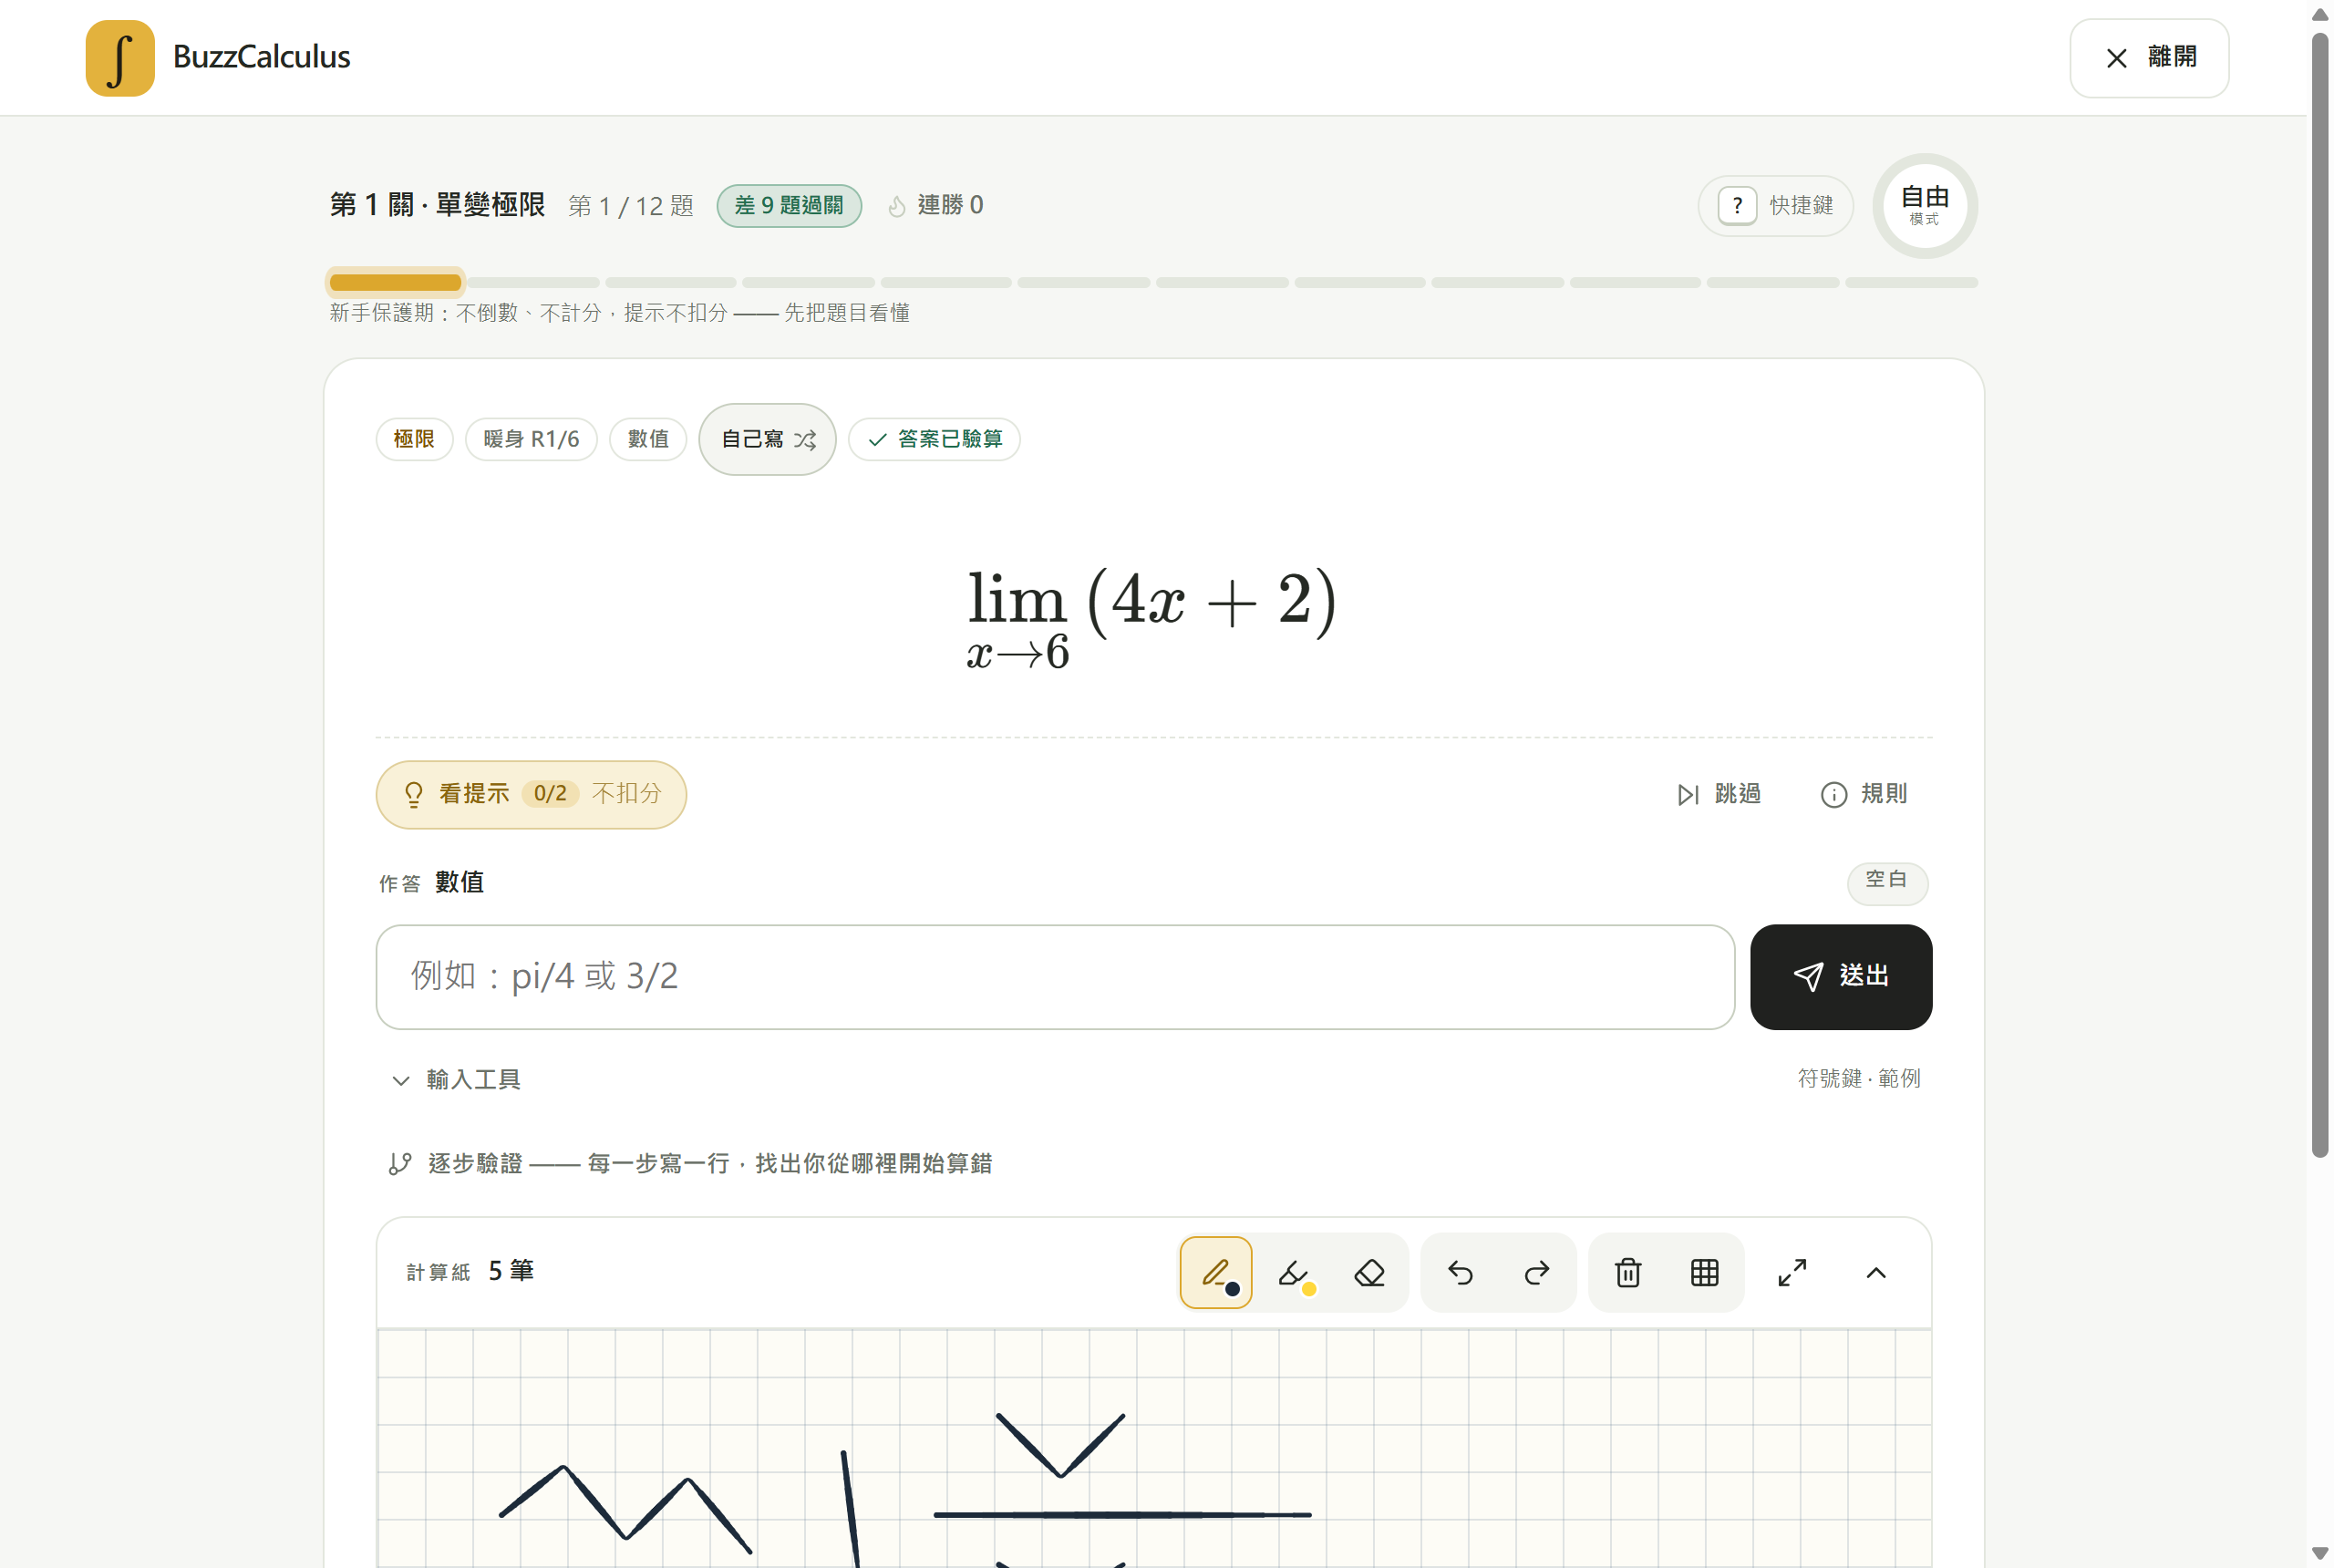
\includegraphics[width=0.78\textwidth]{quiz-board}
\caption{自己寫答案的作答畫面（桌機，攤開了計算紙）。下方的輸入框收到的就是這一章要處理的字串：WebWork 語法、LaTeX、Unicode 與隱式乘法全部混在一起。}
\end{figure}

\section{正規化管線}
\code{normalizeExpression(source, variables)} 依序做這些事，順序有意義：

\begin{enumerate}[label=\arabic*.]
  \item 去掉 \code{\textbackslash left}、\code{\textbackslash right}；\code{\textbackslash cdot} 變 \code{*}。
  \item \textbf{分數}：\code{\textbackslash frac\{a\}\{b\}} 變 \code{((a)/(b))}。用自己的 \code{readGroup} 讀大括號（要處理巢狀），不用正規式。
  \item \textbf{次方群組}：\code{\string^\{n+1\}} 變 \code{\string^(n+1)}。
  \item \textbf{自然指數}：\code{e\string^\{2x\}}、\code{e\string^(x)}、\code{e\string^x} 一律變 \code{exp(…)}。這一步要在把 \code{e} 換成常數 \code{E} 之前做，否則 \code{E**x} 也能算，但 \code{e\string^\{-x\}} 這種帶大括號的會壞。
  \item LaTeX 函數名：\code{\textbackslash sin(} 變 \code{sin(}、\code{\textbackslash ln(} 與 \code{\textbackslash log(} 都變 \code{log(}、\code{\textbackslash arctan(} 變 \code{atan(}，其餘同理。
  \item Unicode：$\pi$ 變 \code{pi}，$\infty$ 變 \code{Infinity}。
  \item 純文字別名：\code{ln} 變 \code{log}，\code{arcsin} 變 \code{asin}……
  \item \textbf{不加括號的函數引數}：\code{sin x} 變 \code{sin(x)}、\code{sqrt 2} 變 \code{sqrt(2)}、\code{cos pi} 變 \code{cos(pi)}。規則：函數名後面接一個原子（單一字母、數字、或 \code{pi}），就把它包起來；接的是括號就照原樣。前面若是數字或右括號，補一個 \code{*}。
  \item \code{\string^} 變 \code{**}；\code{pi} 變 \code{PI}；獨立的 \code{e} 變 \code{E}；去掉所有空白。
  \item \textbf{一元負號與次方}：\code{-x**2} 在 JavaScript 裡是語法錯誤（一元負號與 \code{**} 的結合律未定義），而數學上 $-x^2$ 是 $-(x^2)$。\code{normalizeUnaryPower} 找出「位於一元位置的減號 + 原子 + \code{**} + 原子」，改寫成 \code{-(x**2)}。
  \item \textbf{隱式乘法}：數字或右括號後面接字母或左括號補 \code{*}；右括號後面接數字補 \code{*}；\code{PI}、\code{E} 後面接字母補 \code{*}；黏在一起的識別字（\code{xy}、\code{2xsin}）依「已知變數名，最長優先」切開；識別字後面接左括號、而它不是函數名，補 \code{*}（\code{x(x+1)} 是乘法，\code{sin(x)} 是呼叫）。
  \item \textbf{白名單}：剩下的字元只能是 \code{0-9 a-z A-Z \_ + - * / ( ) . ,}；出現 \code{constructor}、\code{window}、\code{Function}、\code{=>}、\code{;}、\code{=} 任何一個就整個拒收。
\end{enumerate}

\begin{table}[h]
\centering\small\sffamily
\begin{tabularx}{\textwidth}{@{}lY@{}}
\toprule
輸入 & 正規化之後 \\
\midrule
\code{2x\string^3} & \code{2*x**3} \\
\code{\textbackslash frac\{6x\string^3\}\{3\}} & \code{((6*x**3)/(3))} \\
\code{e\string^\{-x\} sin x} & \code{exp(-x)*sin(x)} \\
\code{-x\string^2} & \code{-(x**2)} \\
\code{x(x+1)} & \code{x*(x+1)} \\
\code{2 pi / 3} & \code{2*PI/3} \\
\code{xy + yz}（變數 x、y、z） & \code{x*y+y*z} \\
\code{sqrt 2} & \code{sqrt(2)} \\
\code{x; alert(1)} & （拒收） \\
\bottomrule
\end{tabularx}
\caption{正規化的實際行為。最後一列是白名單在守：求值用的是 \code{new Function}，字串進去之前必須確定裡面只有數學。}
\end{table}

\section{求值}
正規化之後的字串交給 \code{new Function(...names, body)}，\code{body} 先把 \code{Math} 的函數解構出來，再補 \code{sec}、\code{csc}、\code{cot}。任何例外（語法錯、除以零得到的 \code{NaN} 之外的錯）都回傳 \code{NaN}，由上層決定「讀不懂」還是「沒有定義」。

\begin{decision}[用 new Function 而不是自己寫求值器]
判分器需要的是「快、正確、支援所有初等函數」，JavaScript 引擎本身就是最好的求值器。安全性靠兩層：識別字白名單（不在名單裡的識別字直接 \code{NaN}）與字元白名單（只准數學符號）。證明引擎（第二部）反而自己寫了遞迴下降解析器，因為它需要知道「未知符號是哪一個」來給出「\code{y} 沒有宣告」這種訊息。
\end{decision}

\chapter{型別分派}
每一題有一個 \code{answerKind}，\code{checkAnswer(problem, input)} 只做分派：

\begin{table}[h]
\centering\small\sffamily
\begin{tabularx}{\textwidth}{@{}llY@{}}
\toprule
answerKind & 題數 & 判法 \\
\midrule
numeric & 1,356 & 兩邊求值，相對容差 $10^{-6}$；\code{DNE} 特判 \\
expression & 317 & 多點代入（第 5 章） \\
antiderivative & 142 & 去常數後比增量（第 6 章） \\
text & 100 & 正規化後與允許的答案清單比 \\
set & 17 & 解析成多重集合，排序後逐元素比 \\
interval & 16 & 解析成區間串，比端點與開閉 \\
worksheet & 22 & 每格一個子判分 \\
graph / graphtap / graphslope & 24 & 字串相等 / 貪婪最近鄰配對 / 斜率容差 \\
\bottomrule
\end{tabularx}
\caption{十種答案型別與它們的判法。沒有列到的型別回「這個題型目前不能自動判分」，不猜。}
\end{table}

空輸入在分派之前就擋掉：「沒有輸入答案」。這句話跟「數值不對」必須分開——前者是逾時或跳過，不進錯題本的錯因統計。

\chapter{數值題}
\code{checkNumeric(expected, input)}：
\begin{enumerate}[label=\arabic*.]
  \item 先看 \code{DNE}：輸入正規化後是 \code{dne}、\code{doesnotexist}、「不存在」任一，判定「標準答案是不是也是 DNE」，訊息「已用 DNE 判定」。極限不存在是一個合法答案，題庫裡有 7 題 numeric 的答案就是它。
  \item 兩邊各求值。任一邊不是有限數，回「我讀不懂這個數值格式。可以用 pi/4、sqrt(2)、log(2) 這類寫法」——這是格式問題，不是判錯。
  \item 容差 $\max(10^{-7}, 10^{-6}|a|)$，$a$ 是標準答案的值。
  \item 錯的話附一句由 \code{numericDistractorReason} 推出的理由（第 9 章）。
\end{enumerate}

容差為什麼是相對的：答案是 $e^{10}$ 時，絕對容差 $10^{-7}$ 會把 \code{22026.4658} 判錯；答案是 $10^{-8}$ 時，相對容差會把 0 判對——所以兩者取大。$10^{-6}$ 比式子題的 $10^{-5}$ 嚴，因為數值題學生常打小數，六位小數是合理的精度要求。

\chapter{式子等價：多點代入}
\section{演算法}
\begin{lstlisting}
function checkExpression(expected, input, variable, domain) {
  const variables = Array.isArray(variable) ? variable : [variable];
  const samples = expressionSamples(variables).filter((vars) => inDomain(domain, vars));
  let valid = 0;
  for (const vars of samples) {
    const a = evaluateExpression(expected, vars);
    const b = evaluateExpression(input, vars);
    if (!Number.isFinite(a)) continue;               // reference undefined here: skip the point
    if (!Number.isFinite(b)) return wrong("undefined at " + vars);
    valid += 1;
    const tolerance = Math.max(1e-6, Math.abs(a) * 1e-5);
    if (Math.abs(a - b) > tolerance) return wrong("differs at " + vars);
  }
  return { correct: valid >= 3, message: valid >= 3 ? "ok" : "could not parse reliably" };
}
\end{lstlisting}
四個細節：
\begin{itemize}
  \item 標準答案在某點沒定義（$\ln x$ 在負數）就跳過那一點，不算學生的錯；學生的式子在標準答案有定義的點沒定義，才判錯，而且訊息會說在哪一點。
  \item 至少三個點兩邊都有定義才算「判得穩」；不到三個回「格式讀不穩」——例如學生打了一個只在很窄範圍有定義的式子。
  \item 容差 $\max(10^{-6}, 10^{-5}|a|)$，比數值題寬一級：式子的取樣點是無理數附近的值，求值本身有捨入。
  \item 一個點不合就立刻回傳，不再往下比：訊息要指得出是哪一點。
\end{itemize}

\section{取樣點}
\begin{figure}[h]
\centering
\begin{tikzpicture}[x=1.55cm]
  \draw[line width=0.8pt,color=muted,-{Latex[length=2mm]}] (-2.6,0) -- (3.9,0);
  \foreach \x in {-2,-1,0,1,2,3} { \draw[color=muted] (\x,0.08) -- (\x,-0.08); \node[below=2pt,font=\scriptsize\color{muted}] at (\x,0) {\x}; }
  \foreach \x in {0.3137,0.7211,1.2345,1.9871,3.3013,-0.6180,-1.3247,-2.1069} { \fill[gold] (\x,0) circle (2.4pt); }
  \foreach \x in {0.5,1,2} { \draw[rust,line width=0.9pt] (\x,-0.22) -- (\x,0.22); }
  \node[above=5pt,font=\scriptsize\color{rust}] at (1.4,0.3) {避開的「漂亮數」};
  \node[above=5pt,font=\scriptsize\color{gold}] at (-1.3,0.3) {負數：分開 $\sqrt{x^2}$ 與 $x$};
\end{tikzpicture}
\caption{單變數的八個取樣點：$0.3137,\ 0.7211,\ 1.2345,\ 1.9871,\ 3.3013,\ -0.6180,\ -1.3247,\ -2.1069$。}
\end{figure}

\begin{pitfall}[全正的取樣點]
第一版的取樣點全在 $0.35$ 到 $4.4$ 之間。那有一個很實際的漏洞：$\sqrt{x^2}$ 和 $x$ 在正數上完全一樣，但它們不是同一個函數；$|x|$ 與 $x$ 同理。加入負值之後才分得開。同時把「好看的數字」換成無理數附近的值：在 $0.5$、$1$、$2$ 這種點上不同的函數剛好撞在一起的機率高得多（$\sin(\pi/6) = 1/2$ 這類巧合）。
\end{pitfall}

多變數的取樣：每個座標獨立由線性同餘產生器產生（種子固定 20260914，所以每次判分結果一致），24 個點，每個座標取上面八個值之一再加一點擾動。不能把所有點都放在 $y = x + c$ 一條直線上——否則 $x - y$ 與常數分不開。

\section{定義域}
題目可以帶 \code{domain: \{ variable, operator, value \}}；沒帶的話從題幹尾巴讀：\code{,\textbackslash\ x>0}、\code{\textbackslash quad(x\textbackslash ge 1)} 這種寫法由一條正規式 \code{DOMAIN\_TAIL} 抓出來。取樣點先過濾：$x > 0$ 的題不拿負數點去為難只需要在正數成立的答案；反過來，題目沒限制而學生的答案只在正數對，負數點就會抓到。

\begin{decision}[線上判分與離線驗算共用同一套定義域語法]
獨立驗算器（\file{tools/lib/verify\_engine.js}）的 \code{stripDomain} 與這條正規式必須一致，否則會出現「離線驗算說對、線上判分說錯」。這是兩份程式碼共享一個約定的例子，用註解互相指向對方。
\end{decision}

\chapter{不定積分：比增量}
反導函數差一個常數也算對，所以不能直接比 $F(x)$。
\begin{enumerate}[label=\arabic*.]
  \item 先去掉學生寫的 \code{+ C} 或 \code{- C}（\code{stripConstant}，大小寫不分）。
  \item 在取樣點上兩邊求值，收集 $(a_i, b_i)$；標準答案沒定義的點跳過；至少三個點。
  \item 取第一個點當基準，對每一個後續的點驗
  \[
    \bigl|(b_i - b_0) - (a_i - a_0)\bigr| \le \underbrace{\max\bigl(10^{-5},\ 10^{-5}\,|a_i - a_0|\bigr)}_{\text{容差}} + \underbrace{4\varepsilon_{\text{mach}}\max(|b_i|,|b_0|)}_{\text{捨入保護}}
  \]
  \item 捨入保護大於容差時（學生寫了 \code{+ 10\string^20}），明講「積分常數太大，無法可靠比較。請省略常數或改寫成 +C 再送出」。
\end{enumerate}
容差由標準答案的變化量 $|a_i - a_0|$ 決定，不能被學生寫進去的常數放大——這是這個方法的核心：常數在相減時消掉，剩下的差只跟函數本身有關。

\begin{example}[$\int 6x^2\,dx$]
標準答案 \code{2*x\string^3}。學生 \code{2x\string^3+100}：每一點的增量都與 $2x^3$ 相同，正確。學生 \code{x\string^3}：增量是標準的一半，判錯，附「像是係數少了一半」——因為 \code{x\string^3} 正規化後等於 \code{(2*x\string^3)/2}。學生 \code{6x\string^2}：那是被積函數本身，增量對不上，判錯，附「檢查微分回去是否得到原 integrand」。
\end{example}

\chapter{集合、區間、文字、圖形}
\section{集合}
「求所有臨界點」的答案是一組數，順序無所謂。\code{parseNumberSet}：
\begin{itemize}
  \item 空集合是合法答案：\code{\{\}}、「無」、「沒有」、\code{none}、\code{empty}、$\varnothing$ 都解析成空陣列。「這個函數沒有極大值」必須表達得出來，而且不能被判成格式錯。
  \item 去掉大括號與 \code{x =} 這種前綴；用逗號、分號、頓號切；每一段各自求值（元素可以是 \code{pi/3}、\code{sqrt(2)}）；排序。
  \item 比對：個數不同先講「你給了 2 個，答案有 3 個」；個數相同再逐元素以相對容差 $10^{-6}$ 比。
\end{itemize}

\section{區間}
\code{parseIntervals} 要處理 \code{(-inf, 2) U [3, 5]}：
\begin{itemize}
  \item 空區間合法（「沒有凹向下的區間」）。
  \item $\cup$、\code{\textbackslash cup} 都變 \code{U}；去空白；用 \code{U} 切成段。
  \item 每一段：頭尾各取一個括號，中間按\textbf{深度 0 的逗號}切開。這一條是踩過坑才改的：端點本身可以含括號（\code{sqrt(3)/3}、\code{log(2)}），用「不含右括號的字元類」去抓會在 \code{sqrt(3)/3} 上直接失敗，而使用者會看到「參考答案格式有問題」，明明是判分器讀不動。
  \item 端點：\code{inf}、\code{infty}、\code{infinity}、$\infty$ 及其負號變 $\pm\infty$，其餘求值；$lo > hi$ 拒收。
  \item 比對順序：段數不同、端點不同、開閉不同——三句不同的訊息。開閉是這個題型的重點，端點對了但開閉錯代表沒搞清楚端點屬不屬於定義域，那正是題目要考的。
\end{itemize}

\section{文字判定}
收斂、發散、條件收斂、絕對收斂、DNE，含中英別名。\code{normalizeText} 去空白、轉小寫；題目帶一個允許清單 \code{answers} 與顯示用的 \code{canonical}。錯了直接給參考答案——文字判定沒有「差一點」。

\section{圖形題}
\begin{itemize}
  \item \textbf{選圖}：選項本身是圖，作答的值是那條曲線的式子（不是 A/B/C/D，因為選項會洗牌，位置不能當答案）。比對是正規化空白後的字串相等，不做數學等價：這裡問的是「你選到的是不是那一張」。錯的選項可以自帶 \code{why}。
  \item \textbf{點位}：答案是一串 $x$ 座標。判分是貪婪最近鄰配對：對每個目標找最近的、還沒用過的標記，距離在容差內（預設 0.35，題目可調）就配對，否則算漏。標記數與目標數不同先講「要標 3 個位置，收到 2 個」。
  \item \textbf{切線}：答案是斜率，容差 $\max(0.25, 15\%)$——拖出來的東西本來就有手感誤差，這題考的是「看得出切線的方向」不是「拖得準到小數點」。
\end{itemize}

\chapter{選擇題：誘答與理由}
選擇題不用判分，但選項怎麼來決定了它有沒有鑑別力。這一章是判分器的另一半：\textbf{用判分器來造題}。

\begin{figure}[h]
\centering
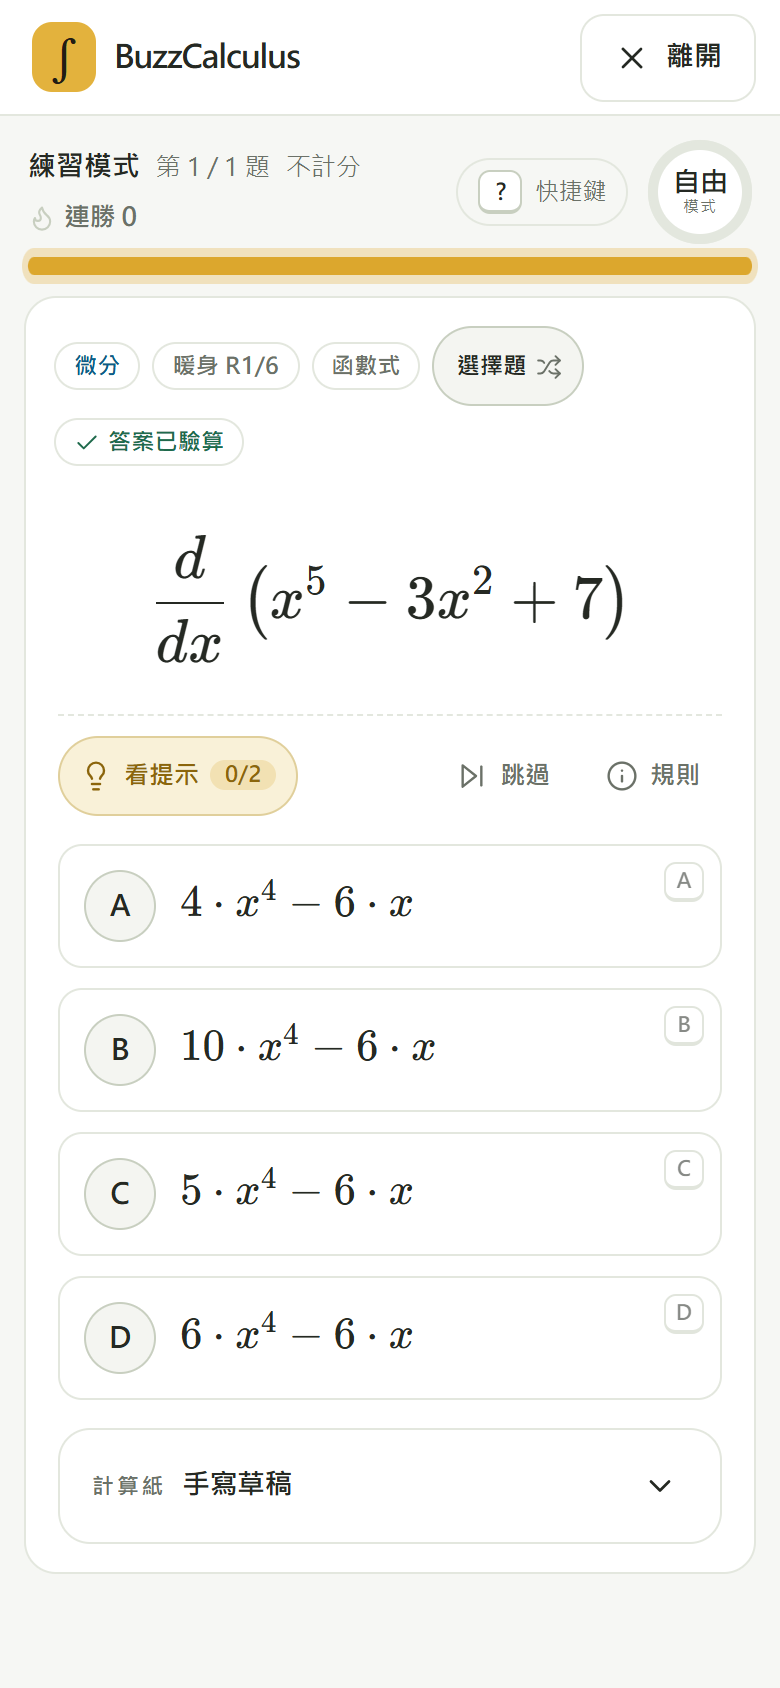
\includegraphics[width=0.36\textwidth]{phone-quiz}
\caption{手機上的選擇題。四個選項之中三個是這一章的產物：它們得像真的犯錯方式、算得出來、量級與長相都跟正解同族，否則排除法零秒答對。}
\end{figure}

\section{誘答的來源，依優先序}
\begin{enumerate}[label=\arabic*.]
  \item \textbf{題目自帶}（\code{distractors}）：「誘答必須是特定幾個選項」的題型。有自帶就不再從別處抓。
  \item \textbf{微擾}（\code{mutatedDistractorLabels}）：把摺疊後的正解裡的數字做 $n+1$、$n-1$、$2n$，最多動前三個數字；再加一個整體變號。每一個都是真實的犯錯方式：鏈鎖忘乘、冪次差一、常數記錯。
  \item \textbf{包裹式}（\code{generatedChoiceDistractors}）：$-(\cdot)$、$2(\cdot)$、$(\cdot)/2$、$(\cdot)+x$、去掉外層係數、去掉像是鏈鎖律的因子。
  \item \textbf{別題的答案}：同型別、同主題優先。真實答案比亂數更像誘答，但要三道過濾（下一節）。
  \item \textbf{保底清單}：\code{0}、\code{1}、\code{x}、\code{sin(x)}……只在沒有自帶誘答且前面湊不滿四個時用。
\end{enumerate}

\section{每一個候選都要過的檢查}
\begin{itemize}
  \item 不能跟正解等價：\code{checkAnswer(problem, value)} 判對的直接丟掉——同一題可能有兩種寫法。
  \item 不能跟已經收的選項等價。
  \item \textbf{算得出來}（\code{wellFormedDistractor}）：字串手術偶爾做出 \code{*y+y*cos(y)}、\code{(…)/x,y,z} 這種東西。規則：不能以運算子開頭或結尾、不能有連續運算子、不能有空括號、括號要配對、代一組固定值要能算出有限數。初學者看到壞掉的式子會以為網站壞了。
  \item \textbf{量級}（\code{numericallyPlausibleDistractor}）：正解的 25 倍以上或 1/25 以下的丟掉。梯子問題的答案是 3/4，選項裡冒出 94586（別題的答案）不會讓人猶豫，只會讓人一眼認出哪個是亂放的，四選一變三選一。反向也擋：正解是 13 位數時，4 和 22/5 一眼就是湊數。
  \item \textbf{格式同族}：正解是精確形（\code{15/2}、\code{pi/4}）時，\code{0.5772156649} 這種長小數一看就是別題漂來的（那還真的是 Euler $\gamma$）。
  \item \textbf{同形}（\code{sameShape}）：同一組變數、長度在正解的 0.4 到 1.8 倍之間。走查初學者流程抓到的：$\frac{d}{dx}(4x^3)$ 的選項是 $(\log x)^{\log x}\cdots$、$2xy + y\cos(xy)$——從不相干的題漂來的外星人，靠排除法零秒答對。
\end{itemize}

\section{選項的長相}
顯示用的 label 做常數摺疊（\code{simplifyChoiceLabel}）：正解照模板原樣印出 \code{5*3/(3-1)}、\code{4\string^2/2} 這種「一看就是公式套出來的」形狀，等於直接洩題。摺疊規則：純整數乘積摺成一個數（但 \code{2*3\string^2} 不能摺成 \code{6\string^2}）；係數 1 不寫；純數字括號只折整數（不把 \code{(1/3)} 折成 \code{0.333}）；不含變數的式子若能寫成分母不超過 3600 的分數就寫分數（連分數逼近），否則保留精確形——帶 $\pi$、$\sqrt{\ }$ 的無理數不硬轉小數。

\begin{pitfall}[反向洩題]
第一版把包裹式誘答排在前面：\code{2*(log(1+e\string^\{x\string^2\})/2)}、\code{(答案)+x} 這種模板包裹折不掉，四個選項裡「唯一乾淨的那個」就是正解——比不折還好認。現在微擾在前、包裹式墊底，而且產生的順序本身是優先序，不能洗牌：洗過一次之後 Boss 題的四個選項變成 $2\cdot X$、$X+1$、$X$、$-5.33$，$X$ 就是答案。四個選項最後才用 \code{quiz.startedAt + problem.id + index} 當種子洗牌位置。
\end{pitfall}

\section{答錯之後：說得出你是怎麼錯的}
\code{choiceDistractorReason} 依序比對：整體變號→「像是符號相反」；乘 2 →「係數多乘一倍」；除 2 →「係數少了一半」；去外層係數→「漏掉外層係數」；去鏈鎖因子→「漏掉鏈鎖律或換元係數」；多了 $\pm x$ →「多加了不該有的項」。數值題再交給 \code{numericDistractorReason}，它的順序即優先序：先驗結構性的錯（負號、倒數、平方、開根號），再驗係數（$\times 2$、$/2$、$\times 3$、$/3$、$\times\pi$、$/\pi$、$\pm 1$、$\times e$、$/e$、$\log$、$\exp$）。每一條都要能一句話說出「你是怎麼走到這個值的」，說不出來的不加；走到最後仍對不上，回「這個值和正確答案對不上；回頭檢查第一步的判型」——說不知道比斷言一件系統不知道的事誠實。

\chapter{測試：判分器怎麼被釘住}
\section{固定案例}
\file{validate\_answer\_checker.js} 用真實的載入順序（照 \file{index.html} 的文件順序載所有 \file{src/*.js}，否則校準走的是後備路徑、驗到的難度跟使用者看到的不一樣）建出判分器，對一組手寫的題目與輸入逐一斷言：反導函數 \code{tan(x)} 對 \code{tan(x)+C}、\code{tan(x)+5}；導數 \code{2*x} 對 \code{2x}、錯 \code{x\string^2}；數值 \code{pi/4} 對 \code{atan(1)}；級數 \code{(exp(1)-exp(-1))/2} 對 \code{sinh(1)}；商法則的分式；多變數的混合偏導；三變數的散度……每一組都同時有該對與該錯的輸入。

\section{黃金檔}
\file{validate\_golden.js} 錄下判分器在固定輸入上的完整輸出（含訊息）；改動取樣點、容差或訊息文字，比對就紅。這比單元測試更「笨」，也更誠實：任何行為變化都得被看見、被解釋。

\section{標準答案本身}
判分器只保證「跟標準答案一致」。標準答案由另一支獨立驗算器把關：從題幹推出一條與解題無關的數值路徑（導數用數值微分、不定積分微分回去、定積分與極限直接算），目前 1,753 題通過，不符數在 CI 裡必須為零。這一部分在《BuzzCalculus 的引擎》第 5 章有完整說明。

\chapter{已知限制}
\begin{itemize}
  \item \textbf{有限取樣不是證明}。兩個不同的函數在八個點上相等的機率極低但不是零。實務上沒有出現過，但程式碼第一行寫著這句話，文件也要寫。
  \item \textbf{定義域不同的等價式}：$\frac{x^2-1}{x-1}$ 與 $x+1$ 在取樣點上相等（取樣點避開 1），判對。這是有意的：反導函數與化簡結果常常差一個可去點，判錯會冤枉大多數人。
  \item \textbf{分段函數}：輸入語言不支援 \code{if}，題庫也沒有這種答案。
  \item \textbf{複數}：$\sqrt{-1}$ 得 \code{NaN}，會被當成「沒有定義」。
  \item \textbf{變數名}：只認題目宣告的變數；\code{t} 的題打 \code{x} 會被當未知識別字判成讀不懂，訊息會提示寫法。
\end{itemize}

% ═══════════════════════════════════════════════════════
\part{白話證明}
% ═══════════════════════════════════════════════════════

\chapter{問題與三分之二的誠實}
\section{要判的東西長什麼樣}
\begin{example}[題目與一份參考證明]
題目：用 $\varepsilon$–$\delta$ 定義證明 $\lim_{x\to 2} 3x = 6$。
\begin{quote}
任取 $\varepsilon > 0$。\\
取 $\delta = \varepsilon/3$。\\
假設 $0 < |x - 2| < \delta$。\\
則 $|3x - 6| = 3|x - 2| < 3\delta = \varepsilon$。\\
所以 $\lim_{x\to 2} 3x = 6$。
\end{quote}
\end{example}
\begin{figure}[h]
\centering
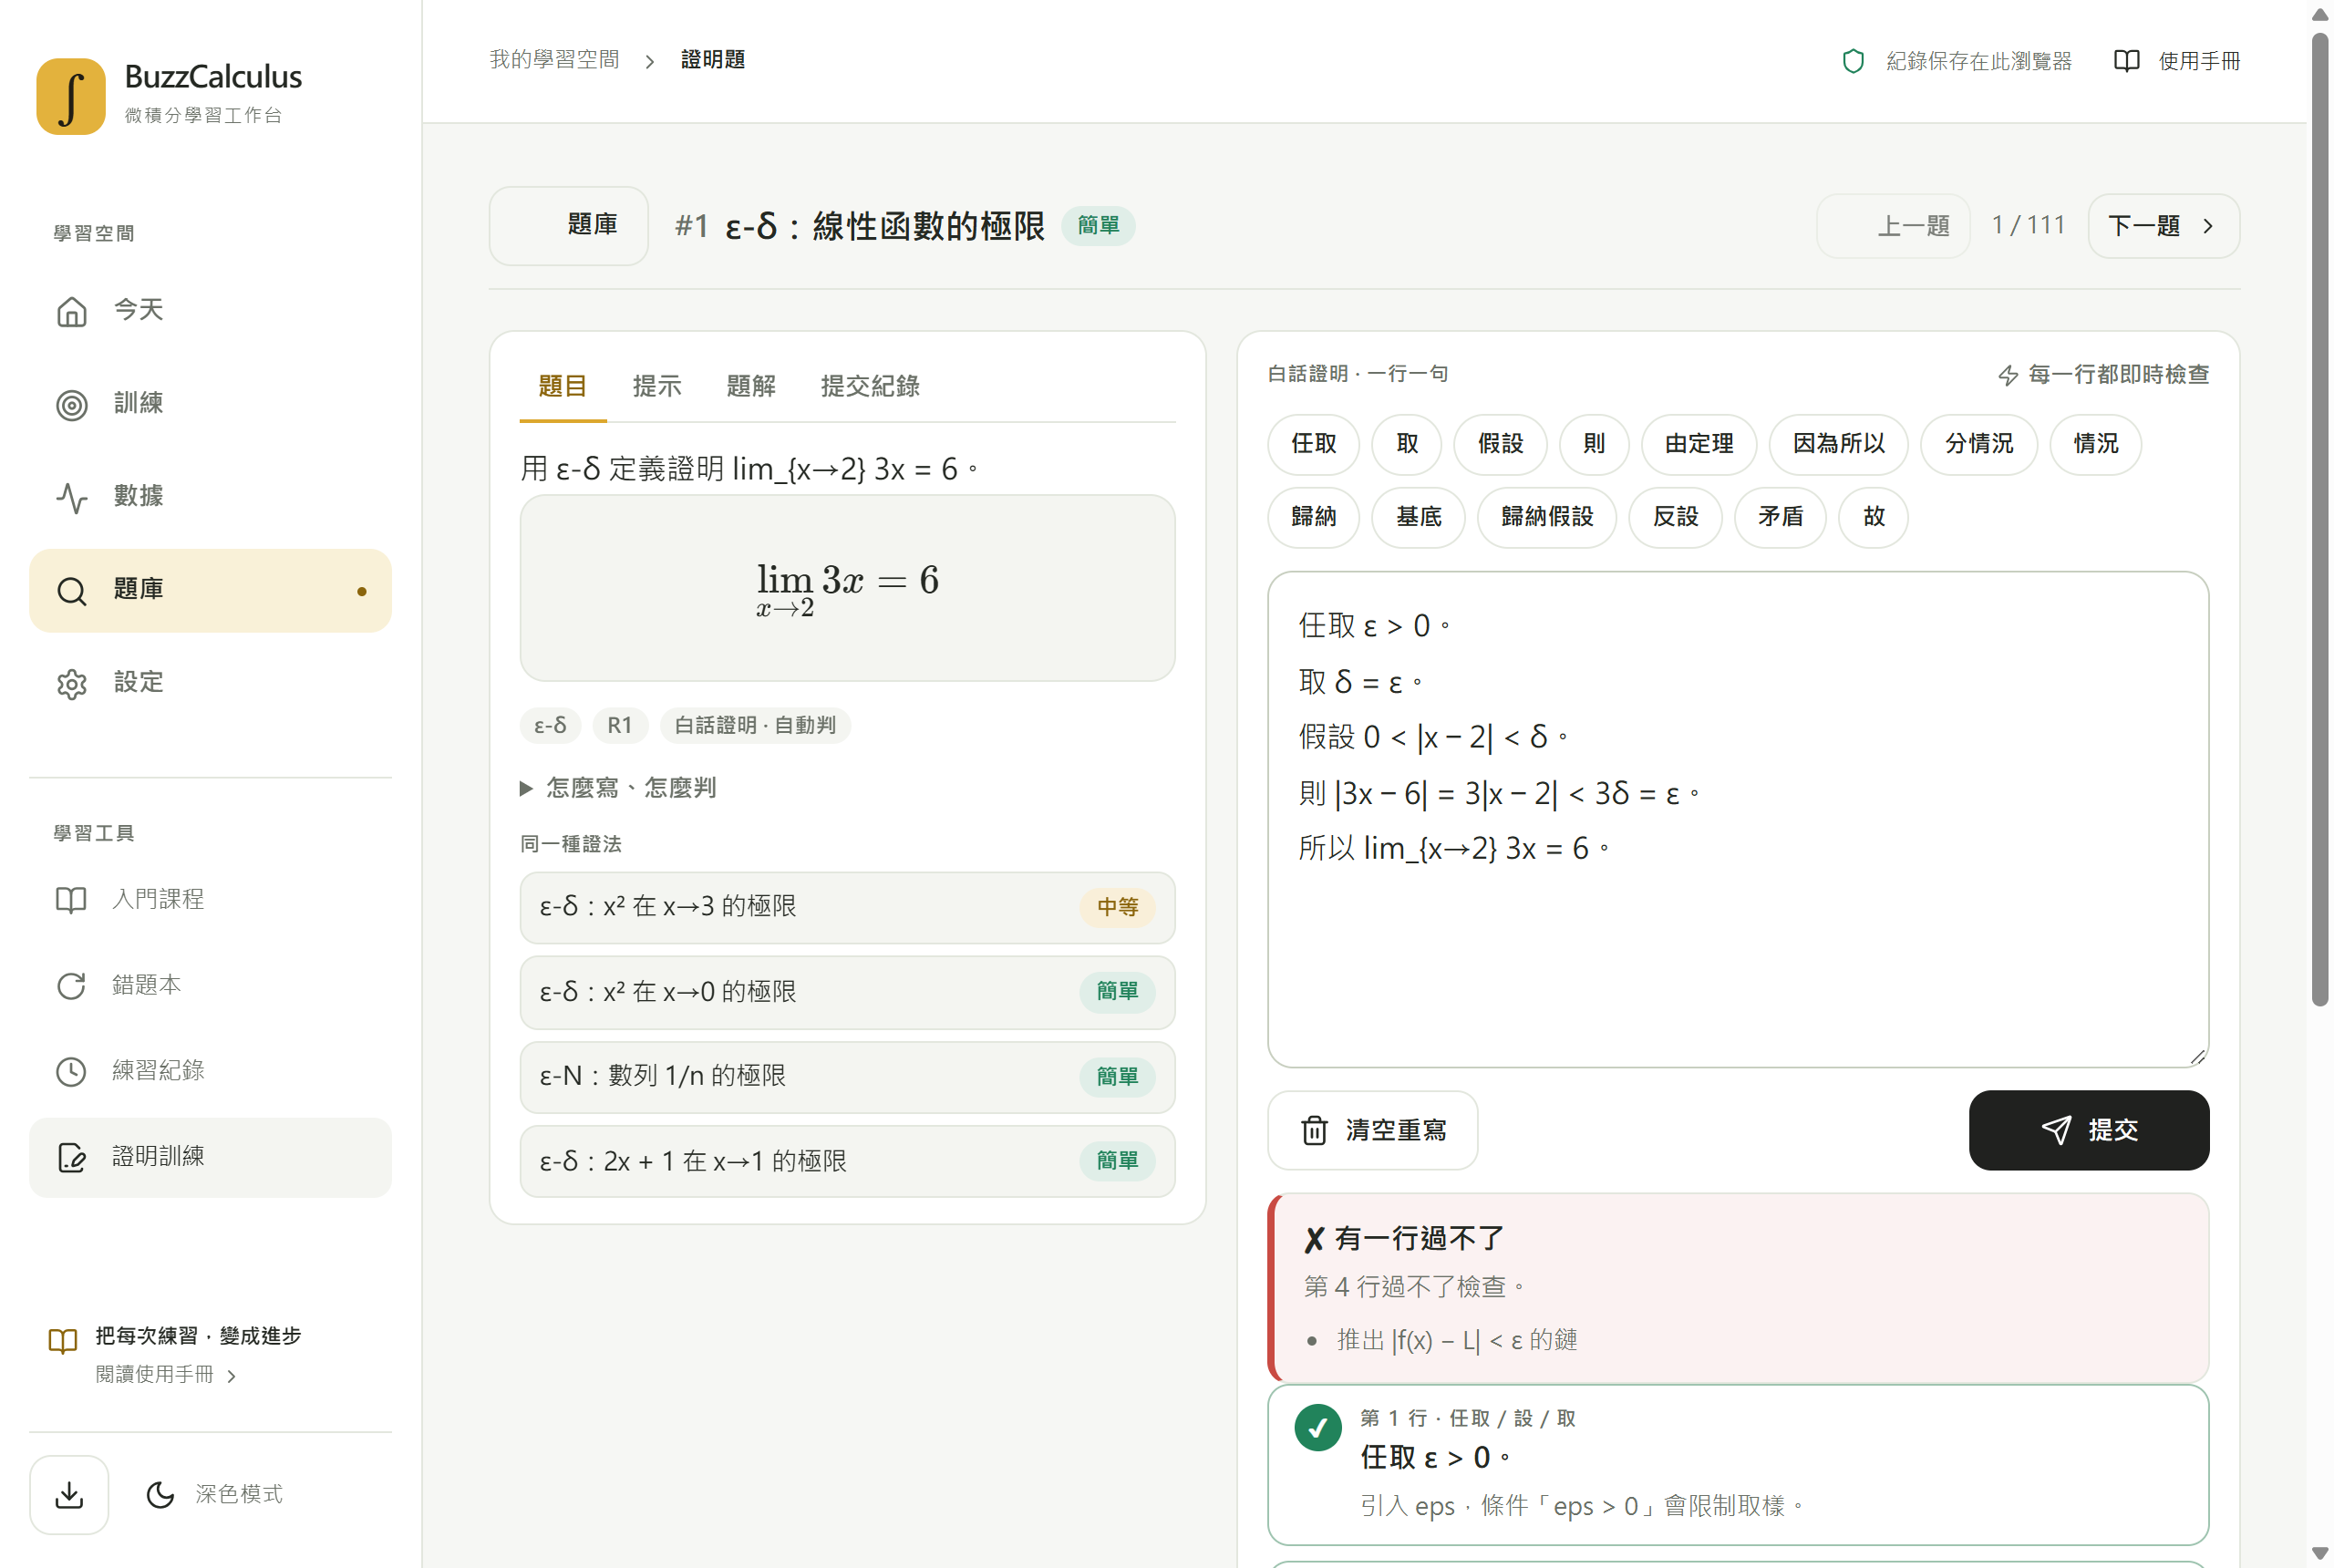
\includegraphics[width=0.92\textwidth]{proof-editor}
\caption{白話證明編輯器。左邊是使用者打的證明（這一份把 $\delta$ 取成 $\varepsilon$），右邊是逐行的三色報告：紅在第 4 行，並列出反例的取值。}
\end{figure}

五行、四種句型、一條三段的代數鏈、一個目標。學生會寫的變體：$\delta$ 取錯、假設漏掉 $0 <$、鏈的方向寫反、跳過中間一段、最後一句跟目標對不上、一行塞兩句、用了沒宣告的變數。檢查器要對每一種給出對的行號與對的理由。

\section{做得到的三分之二}
\begin{enumerate}[label=\arabic*.]
  \item \textbf{句型引擎}：認得這句話在做什麼——設變數、假設、代數推導、引用定理、分情況、歸納、下結論。
  \item \textbf{代數引擎}：$A = B \le C < D$ 這種鏈，在目前的假設下隨機取點驗；等式看差、不等式看方向。
  \item \textbf{推論引擎}：一小本規則字典（均值定理、三角不等式、夾擠……），比對「你寫的句子」跟「規則會吐出的形狀」，並檢查定理的前提有沒有在前面出現。
\end{enumerate}
剩下的三分之一——存在句、抽象函數 $f$、數論——標黃：看得懂但驗不了，不假裝。

\section{三色的語意}
\begin{itemize}
  \item \ok：驗過成立。代數鏈在取樣點上成立、規則形狀對上、骨架角色到位。
  \item \bad：驗過不成立，或違反硬規則（一行兩句、裸關係式沒有句型、沒宣告的變數、還沒反設就說矛盾、還沒對上目標就得證）。
  \item \unsure：看得懂但驗不了。抽象函數、規則字典裡沒有的定理、數值上成立但跟前面接不上的鏈、文字主張。
\end{itemize}
最後的判定五種：\code{empty}、\code{broken}（有紅）、\code{incomplete}（骨架缺角色）、\code{partial}（有黃沒紅）、\code{verified}（全綠且骨架完整）。

\section{題目規格}
每一題是一個物件，引擎只認這些欄位：
\begin{table}[h]
\centering\small\sffamily
\begin{tabularx}{\textwidth}{@{}lY@{}}
\toprule
欄位 & 意義 \\
\midrule
\code{vars} & 變數與取樣範圍：\code{\{ x: \{min:-4, max:8\}, eps: \{min:0.05, max:2\} \}}；可標 \code{int} \\
\code{goal.text} & 目標的文字寫法清單（$\lim$ 的各種寫法會被 \code{canonicalText} 收斂） \\
\code{goal.relation} & 目標是一條關係式時（\code{x\string^2+1 >= 2x}），用它比對結論、代 $n$ 驗基底 \\
\code{bound} & $\varepsilon$–$\delta$ 的收尾鏈兩端：\code{\{ lhs: "abs(3*x-6)", rhs: "eps" \}}；數列題加 \code{threshold: "N"} \\
\code{skeleton} & \code{direct} / \code{epsilon-delta} / \code{induction} / \code{cases} / \code{contradiction} \\
\code{facts} & 題目給的文字事實（「f 可微」）或帶佔位符的全稱條件（\code{f'(\_) = 0}） \\
\code{given} & 題目一開始就成立的宣告（會先套用 \code{applyDeclaration}） \\
\code{abstract} & 抽象函數與其值域：\code{\{ f: \{min:-3,max:3\}, "f'": \{min:0,max:0\} \}} \\
\code{functions} & 題目提供的可算函數（歸納題的 $S(k)$） \\
\code{macros} & 正規式替換，把使用者的慣用寫法換成引擎認得的 \\
\code{reference} & 參考證明，一行一句；\code{optional} 標可刪的行；\code{allowUnsure} 允許黃 \\
\bottomrule
\end{tabularx}
\caption{規格欄位。\code{reference} 不是給使用者看的答案，是驗證器用來做變異測試的基準（第 22 章）。}
\end{table}

\chapter{正規化}
使用者會混用全形標點、希臘字母、LaTeX 指令與 Unicode 符號。\code{normalize} 做的事：
\begin{itemize}
  \item 全形數字、字母轉半形。
  \item 「，。：；（）「」」轉半形或刪除；$\le\ \ge\ \ne\ -\ \times\ \cdot\ \div$ 轉 ASCII；$\in$ 變 \code{ in }；$\infty$ 變 \code{inf}；$\sqrt{\ }$ 變 \code{sqrt}；$\pi$ 變 \code{pi}；$\varepsilon$ 變 \code{eps}；$\delta$ 變 \code{delta}；$\to$ 變 \code{->}；$\Rightarrow$ 變 \code{=>}；$\forall$、$\exists$ 變 \code{forall}、\code{exists}；上標 $^2$ 到 $^6$、$^n$ 變 \code{\string^2}……；希臘字母 $\xi\ \eta\ \theta\ \lambda\ \mu\ \alpha\ \beta\ \gamma$ 各有名字。
  \item LaTeX：\code{\textbackslash epsilon}、\code{\textbackslash varepsilon} 變 \code{eps}；\code{\textbackslash le}、\code{\textbackslash leq} 變 \code{<=}；\code{\textbackslash cdot}、\code{\textbackslash times} 變 \code{*}；\code{\textbackslash sqrt}、\code{\textbackslash sin} 等去掉反斜線。
  \item 多個空白收成一個。
\end{itemize}
另外兩個常用的變形：\code{compact}（正規化後去所有空白、轉小寫，做字面比對用）；\code{replaceBars}（把不巢狀的 \code{|…|} 翻成 \code{abs(…)}，最多八輪——證明裡九成九的絕對值都不巢狀）。

$\lim$ 有太多寫法：
\begin{center}
\code{lim\_\{x→2\} 3x = 6}\qquad \code{lim x→2 (3x) = 6}\qquad \code{lim\_(x->2) 3x=6}
\end{center}
\code{canonicalText} 把它們收斂成 \code{lim[x->2]3x=6}：抓 \code{lim}、可有可無的底線與括號、變數、箭頭、目標值，重組成固定格式，去乘號，再把緊接的一層括號拆掉。目標比對用這個鍵。

\chapter{表達式引擎}
判分器用 \code{new Function} 求值；證明引擎自己寫解析器，因為它要知道\textbf{哪一個}符號沒宣告。

\begin{figure}[h]
\centering
\begin{tikzpicture}[
  node distance=4mm,
  stg/.style={draw=line,fill=paper,rounded corners=2pt,inner sep=5pt,font=\small\sffamily,align=center,minimum width=26mm,minimum height=9mm},
  ex/.style={font=\scriptsize\ttfamily\color{muted},align=left},
  arr/.style={-{Latex[length=2mm]},color=muted,line width=0.7pt}]
  \node[stg] (a) {normalize};
  \node[stg,right=of a] (b) {replaceBars\\tokenize};
  \node[stg,right=of b] (c) {splitIdentifier};
  \node[stg,right=of c] (d) {隱式乘法};
  \node[stg,right=of d] (e) {遞迴下降\\→ 閉包};
  \draw[arr] (a)--(b); \draw[arr] (b)--(c); \draw[arr] (c)--(d); \draw[arr] (d)--(e);
  \node[ex,below=3mm of a] {3|x−2|＜3δ};
  \node[ex,below=3mm of b] {3 abs ( x - 2 )\\< 3 delta};
  \node[ex,below=3mm of c] {2kh → 2 k h};
  \node[ex,below=3mm of d] {3 * abs(x-2)\\< 3 * delta};
  \node[ex,below=3mm of e] {(env) => 3*|env.x−2|};
\end{tikzpicture}
\caption{一條式子從使用者的字串到可以在取樣點上呼叫的閉包。每一層只做一件事，錯誤訊息才指得出是哪一層看不懂。}
\end{figure}

\section{分詞}
\code{tokenize}：先 \code{replaceBars}、去空白；數字（含小數點）、識別字（字母開頭，可含數字、底線、撇號——$f'$ 是一個識別字）、\code{**} 視為 \code{\string^}、運算子 \code{+ - * / \string^ ( ) ,}。其他字元丟「看不懂的符號『$\ldots$』」，上層轉成「式子裡只能有數學，中文要放在句型的位置」。

\section{黏在一起的識別字}
使用者手寫 \code{2kh} 很自然，但分詞器看到的是一個叫 \code{kh} 的東西。\code{splitIdentifier(name, known)}：不認得的識別字先試著切成「認得的名字」的串（最長優先），切得開就是乘積，切不開照原樣（之後報未知符號）。\code{xsin} 切成 \code{x}、\code{sin}；\code{sqrta} 切成 \code{sqrt}、\code{a}；\code{cosh} 不會被切成 \code{cos}、\code{h}，因為 \code{cosh} 本身是認得的名字，先整個比對。

\section{隱式乘法}
\code{insertImplicitMultiplication}：前一個 token 是「值」（數字、非函數的識別字、右括號）而下一個 token「開始一個值」（數字、識別字、左括號），中間補 \code{*}。例外：函數名後面接左括號是呼叫。所以 \code{3x}、\code{2(x+1)}、\code{k(k+1)}、\code{(a)(b)} 都是乘法，\code{sin(x)}、\code{S(k)} 是呼叫。

\section{文法}
遞迴下降，四層：
\[
\begin{aligned}
\textit{expr} &::= \textit{term}\ ((\texttt{+}\mid\texttt{-})\ \textit{term})^* \\
\textit{term} &::= \textit{unary}\ ((\texttt{*}\mid\texttt{/})\ \textit{unary})^* \\
\textit{unary} &::= \texttt{-}\ \textit{unary} \mid \texttt{+}\ \textit{unary} \mid \textit{power} \\
\textit{power} &::= \textit{atom}\ (\texttt{\string^}\ \textit{unary})^?
\end{aligned}
\]
次方的指數是 \textit{unary}，所以 \code{x\string^-2} 合法；次方在一元負號之下，所以 \code{-x\string^2} 是 $-(x^2)$。原子：數字、括號、函數呼叫（含多參數，\code{min(1, eps/7)}）、函數名後直接接一個原子（\code{sqrt a}、\code{sin x}）、常數（\code{pi}、\code{e}、\code{inf}，但變數名優先）、變數。編譯的結果是一個 \code{(env) => number} 的閉包樹，之後每個取樣點各呼叫一次。

未知符號丟一個帶 \code{unknownSymbol} 的錯誤，上層據此說「『y』沒有宣告。先用『設／任取／取』引入它」。

\chapter{句型}
\section{十三種}
\begin{table}[h]
\centering\small\sffamily
\begin{tabularx}{\textwidth}{@{}llY@{}}
\toprule
kind & 標籤 & 觸發的寫法（節錄） \\
\midrule
qed & 得證 & 得證、證畢、證明完畢、Q.E.D.、$\blacksquare$ \\
induction & 用歸納法 & 用數學歸納法、對 n 做歸納、by induction on n \\
cases / case & 分情況、情況 N & 分兩種情況、考慮三種情況；情況一：$x \ge 0$、case 1: \\
contradiction-start & 反設 & 反設、假設不然、假設結論不成立、suppose not \\
contradiction & 矛盾 & …矛盾、a contradiction \\
base & 當 n = 1 時 & 當 n = 1 時、when n = 1、for n = 1 \\
hypothesis & 假設 n = k 時成立 & 假設 n = k 時成立、suppose n = k holds \\
let & 任取／設／取 & 任取、任意取、給定、固定、設、令、取、let、fix、choose \\
assume & 假設／若…則… & 假設、若、如果、suppose、assume、if；可帶「則」子句 \\
by & 由 <規則>，… & 由、根據、依據、利用、by、using、applying \\
because & 因為…，所以… & 因為…，所以／故／因此；because…, so／hence \\
claim & 則／所以 <推導> & 則、那麼、得、所以、故、因此、於是、即、然後、同理、展開得、整理得 \\
unknown & — & 其餘 \\
\bottomrule
\end{tabularx}
\caption{句型表。順序即優先序：先比特殊的（得證、歸納、分情況、反設），最後才是最寬的「則／所以」。}
\end{table}

中文關鍵字後面可以不空格（「因為x>0，所以x²>0」）；英文的要空格，不然 \code{as}、\code{so} 會咬到 \code{assume}、\code{some}。

\section{兩條硬規則}
\begin{itemize}
  \item \textbf{一行一句}。句號只能在最後。「設 x。則 x² ≥ 0。」要拆成兩行，否則後半句會被當成前半句的一部分。違反直接紅，並說「這一行有 2 句，每一句各自一行」。
  \item \textbf{裸關係式不猜}。一行只有 \code{(x−1)² ≥ 0} 沒有句型，紅：「它是推導（則／所以／故）、引入（設／任取）、還是條件（假設）？三個意思差很多。」
\end{itemize}

\section{一句裡的多個主張}
\code{statementList} 把一句切成主張：深度 0 的逗號與分號切；「且」與 \code{and} 切；每段去掉開頭的「即、也就是說、因為、所以」；「對所有正整數 n」「對任意 x」這種量詞裝飾不是主張，略過。所以「則 $a \ge 0$ 且 $b \ge 0$」是兩個主張，各自驗。

\chapter{條件與取樣}
\begin{figure}[h]
\centering
\begin{tikzpicture}[
  node distance=5mm and 8mm,
  box/.style={draw=line,fill=paper,rounded corners=2pt,inner sep=5pt,font=\small\sffamily,align=center,minimum height=9mm},
  ctx/.style={draw=gold,fill=goldsoft,rounded corners=2pt,inner sep=5pt,font=\small\sffamily,align=left},
  arr/.style={-{Latex[length=2mm]},color=muted,line width=0.7pt}]
  \node[box] (line) {下一行};
  \node[box,right=of line] (cls) {classify\\（十三句型）};
  \node[box,right=of cls] (handle) {對應的 handle\\let / assume / claim / by …};
  \node[box,right=of handle] (verdict) {這一行的\\顏色 + 備註};
  \node[ctx,below=7mm of handle] (ctx) {ctx：vars · defs · constraints · facts · atoms\\asserted · verifiedLinks · knownExprs · run · skeleton};
  \draw[arr] (line)--(cls); \draw[arr] (cls)--(handle); \draw[arr] (handle)--(verdict);
  \draw[arr] (ctx.north) -- node[left,font=\scriptsize\color{muted}]{讀} ($(handle.south)+(-6mm,0)$);
  \draw[arr] ($(handle.south)+(6mm,0)$) -- node[right,font=\scriptsize\color{muted}]{寫} (ctx.north-|{$(handle.south)+(6mm,0)$});
  \coordinate (bot) at ($(ctx.south)+(0,-5mm)$);
  \draw[arr] (verdict.south) |- (bot) -| (line.south);
  \node[below=1mm,font=\scriptsize\color{muted}] at ($(bot)!0.5!(bot-|line.south)$) {summarize：五種判定};
\end{tikzpicture}
\caption{證明引擎的主迴圈。每一行在「到目前為止的上下文」裡驗，驗完把自己的貢獻寫回去；最後由 \code{summarize} 看三色與骨架給判定。}
\end{figure}

\section{上下文}
\code{check} 為每一份證明建一個 \code{ctx}：\code{vars}（宣告過的變數與其範圍）、\code{defs}（定義：$\delta = \varepsilon/3$）、\code{constraints}（條件：$0 < |x-2| < \delta$，各帶 \code{caseId}）、\code{facts}（文字假設）、\code{textFacts}（連續、可微這類鍵）、\code{atoms}（抽象函數的取樣變數）、\code{userFunctions}、\code{asserted}（存在句給的關係）、\code{verifiedLinks}（驗過的關係）、\code{knownExprs}（出現過的式子）、\code{induction}、\code{cases}、\code{contradiction}、\code{skeleton}（角色到位旗標）、\code{run}（跨行的鏈）、\code{goalDone}。每一行處理完就更新它，後面的行在更新後的上下文裡驗。

\section{登記一條關係}
\code{registerRelation(lhs, rhs, op, caseId)}：等式而且不在某個情況裡時，先試著\textbf{解成定義}——連續變數用拒絕取樣永遠碰不到等號，所以 $\delta = \varepsilon/3$ 必須變成「$\delta$ 由 $\varepsilon$ 算出來」而不是「抽一個 $\delta$ 看它等不等於 $\varepsilon/3$」。三種解法：
\begin{itemize}
  \item \code{solveForUnknown}：一邊是還沒定義的變數或抽象 atom，或「那個東西 $\pm$ 別的」（$f(y) - f(x) = f'(c)(y-x)$ 解出 $f(y)$）。
  \item \code{solveLinear}：等式對某一個抽象 atom $u$ 是一次的。用取樣驗「一次」：$E(u) = L - R$，檢查 $E(2) = 2E(1) - E(0)$ 在所有取樣點成立，就解 $u = -E(0)/(E(1)-E(0))$。
  \item 都不行就當條件放進 \code{constraints}。
\end{itemize}

\section{拒絕取樣}
\code{drawSamples(spec, ctx, count)}：
\begin{enumerate}[label=\arabic*.]
  \item 每個變數的範圍：atom 的值域、規格宣告、上下文宣告，都沒有就用預設——\code{eps} 與 \code{delta} 是 $[0.05, 2]$，其餘 $[-3, 3]$；標 \code{int} 的取整數。
  \item 固定種子的線性同餘產生器（規格可給 \code{seed}），所以同一份證明每次的報告一樣。
  \item 每一輪：自由變數各抽一個值；定義按依賴順序求值，定義可能互相引用、登記順序不一定是依賴順序（$f(y)$ 先解出來、$f'(c)$ 後來才 $= 0$），所以多跑幾輪直到每個定義都算得出有限值；然後對每一條當前情況有效的條件驗 \code{RELATION\_TEST}，全過才收。
  \item 最多 $\max(4000, 40\times\text{count})$ 次嘗試。抽不到任何點是一個明確的訊號：假設互相矛盾或條件太緊，會變成黃並說出來；在反證裡它是預期的。
\end{enumerate}
關係的容差：等式 $|a-b| \le 10^{-6}(1+|a|+|b|)$；嚴格不等式留 $10^{-9}$ 的邊。

\chapter{代數鏈：驗與接地}
\section{切鏈與整體方向}
\code{splitChain} 用 \code{<= >= != < > =} 切成 \code{exprs} 與 \code{ops}。\code{chainOverallOp}：全是 \code{=} 就是 \code{=}；只有 \code{=} 與 \code{<}、\code{<=} 就是 \code{<}（有嚴格的）或 \code{<=}；同理 \code{>}；混了 $\ge$ 與 $\le$ 回 \code{null}，這是「方向不一致」的紅：一條鏈只能朝一個方向，兩件事請分兩句。

\section{驗一段}
\code{evaluate(lhs, rhs, op, ctx)}：編譯兩邊（未知符號→紅並指名；看不懂的符號→紅；其他編譯錯→黃），抽 160 個點，逐點驗；任一點不成立立刻回傳反例——只列使用者宣告過的變數與 atom 的值，最多五個，數字取四位有效。全部成立回 \code{checked} 數。\code{verifyChain} 對每一段呼叫它，遇到紅就停。

\begin{example}[$\delta$ 取錯]
「取 $\delta = \varepsilon$」之後，「則 $|3x-6| = 3|x-2| < 3\delta = \varepsilon$」的第三段 $3\delta = \varepsilon$ 在 $\varepsilon = 0.3$ 時左邊 0.9、右邊 0.3，紅在第 4 行——不是第 2 行。第 2 行的設定本身不是錯，錯的是它撐不起第 4 行。
\end{example}

\section{數值上成立不等於推導出來}
一條鏈全段成立之後，還有四道關：
\begin{itemize}
  \item \textbf{兩邊一樣的段}（$x^2+1 = x^2+1$）：不是推導，是用來湊「兩段鏈」的，紅。
  \item \textbf{方向混合}：紅。
  \item \textbf{接地}：鏈要跟前面接得上，否則黃——一行寫出目標就算證完，那不是證明。接地的方式（任一即可）：是前提（因為…句的前半）；引用了規則字典裡的定理；對上目標而且骨架已到齊；第一段是\textbf{顯然的起點}；\code{anchored}：鏈的一端是前面出現過的式子、宣告過的變數、定義、atom、自訂函數代常數、目標的一邊（只認多段鏈的第一個式子，而且第一段本身不能就是目標）；\code{equivalentToKnown}：跟前面某條驗過的不等式等價。
  \item \textbf{跨行的鏈}：這一行的第一個式子等於上一行的最後一個，就併成同一條 run（Bernoulli 的歸納步驟就是兩行）。$\varepsilon$–$\delta$ 的收尾與歸納步驟的判定看的是 run。
\end{itemize}

\section{顯然的起點：符號樹}
「$(a-b)^2 \ge 0$」「$a + b \ge 0$（$a, b \ge 0$）」「$|\sin\theta| \le 1$」「$\sqrt{x} + 2 \ge 2$」是課本上會直接用的起點。\code{isObviousStart} 把 $L - R$ 讀成樹，問一個問題：這個東西是不是一看就 $\ge 0$（或 $> 0$）。\code{signOf} 的規則：
\begin{itemize}
  \item 正常數→正；0→非負；負常數→不知道。
  \item 變數：查它的已知下界（規格範圍、宣告條件 $a \ge 0$、情況條件）；黏在一起的名字拆開（\code{sqrtx} 是 $\sqrt{x}$，\code{ab} 是 $a\cdot b$）。
  \item $\exp$、$\cosh$→正；$|\cdot|$、$\sqrt{\ }$→非負（引數為正則正）。
  \item 偶次方→非負（底為正則正）；其他次方只在底為正時為正。
  \item 積與商：兩邊都有符號才有符號，商的分母必須為正。
  \item 和：兩邊都非負則非負，任一為正則正。
  \item 差：只認減去 0 或負常數。$x^2 + 1 \ge 2x$ 數值上永遠對，但它不是顯然——要展開一個平方才看得到，所以不算。
\end{itemize}

\begin{figure}[h]
\centering
\begin{tikzpicture}[
  level distance=11mm, sibling distance=30mm,
  every node/.style={font=\small},
  n/.style={draw=line,fill=paper,rounded corners=2pt,inner sep=3pt,minimum width=14mm,align=center},
  s/.style={font=\scriptsize\sffamily\color{moss}},
  edge from parent/.style={draw=muted,line width=0.6pt}]
  \node[n] {$+$ \quad \textcolor{moss}{\scriptsize 非負}}
    child { node[n] {$(\cdot)^2$ \quad \textcolor{moss}{\scriptsize 偶次方→非負}}
      child { node[n] {$a-b$ \quad \textcolor{muted}{\scriptsize 不知道}} } }
    child { node[n] {$\sqrt{\cdot}$ \quad \textcolor{moss}{\scriptsize 非負}}
      child { node[n] {$x$ \quad \textcolor{moss}{\scriptsize 宣告 $x \ge 0$}} } };
  \node[font=\small,anchor=west] at (4.2,-0.1) {$(a-b)^2 + \sqrt{x} \ \ge\ 0$ 是顯然的起點};
  \node[font=\small,anchor=west] at (4.2,-1.3) {$x^2 + 1 - 2x$：差，只認減常數 → 不顯然};
\end{tikzpicture}
\caption{\code{signOf} 把 $L - R$ 讀成樹，由葉往上推符號。偶次方、絕對值、根號、指數不需要知道底下是什麼；差只在減去 0 或負常數時才有結論。}
\end{figure}

\section{等價於已知的不等式}
$1 + h \ge 0$ 之於 $h \ge -1$：移項。\code{equivalentToKnown} 把兩條不等式都寫成「大邊減小邊」，在 120 個取樣點上驗兩者成\textbf{固定正比}——移項、乘正數都是這樣；兩條剛好都成立的不等式不是。\code{equivalentToConstraint} 對條件做同一件事。

\chapter{規則字典與文字事實}
\section{規則}
每條規則：名字（中英別名）、它會吐出的句子形狀（正規化後的正規式）、可有的前提 \code{requires}。
\begin{table}[h]
\centering\small\sffamily
\begin{tabularx}{\textwidth}{@{}lYl@{}}
\toprule
規則 & 形狀 & 前提 \\
\midrule
三角不等式 & \code{abs(A+B)<=abs(A)+abs(B)} & — \\
均值定理 & \code{f(b)-f(a)=f'(c)*(b-a)} & 可微 \\
泰勒 & \code{f(a+h)=…f''(ξ)…} & 二次可微 \\
Rolle & \code{f'(c)=0} & 可微 \\
極值定理 & 出現最大值／最小值 & 連續 \\
費馬 & \code{f'(c)=0} & — \\
夾擠 & 出現 lim & 前面有 $A \le B \le C$ 的鏈 \\
算幾不等式 & \code{(a+b)/2>=sqrt(…)} 或 \code{>=2*sqrt(…)} & — \\
中間值定理 & \code{f(c)=…} & 連續 + 兩端異號 \\
導數定義 & 出現 lim & — \\
假設／歸納假設 & （無形狀：拿前面登記的東西用） & — \\
代數／展開／因式分解 & （無形狀：走代數引擎） & — \\
Bernoulli & \code{(1+x)\string^n>=1+…} & — \\
單調性、連續性、Cauchy、二項式定理 & （無形狀） & — \\
\bottomrule
\end{tabularx}
\caption{規則字典。形狀對上就綠；對不上但句子本身能數值驗，就走代數引擎；都不行標黃。}
\end{table}
\code{findRule} 用模糊比對：去掉「定理」「theorem」之後，別名與輸入互相包含即可。不在字典裡的名字變成 \code{unknown} 規則：式子驗過了照樣綠，但備註「『某某』不在我的規則字典裡，但式子本身驗過了」。

\section{前提}
\code{ruleRequirementMissing}：均值定理要 $f$ 可微；中間值定理要 $f$ 連續，而且前面要驗出兩端異號（\code{verifiedLinks} 裡同時有 $\cdot < 0$ 與 $\cdot > 0$）；夾擠要前面出現過 $A \le B \le C$ 的鏈。缺了就黃，訊息說缺什麼、怎麼補（「多項式可以寫『因為 f 是多項式，所以 f 連續』」）。

\section{文字事實}
「$g$ 是多項式」「$f$ 連續」「$f$ 可微」「$f$ 二次可微」算不出來但常被引用，用鍵登記（\code{continuous:f}）。可以推：多項式與可微蘊含連續；二次可微蘊含可微；使用者自己「令 $g(x) = \cos x - x$」的函數，本體只由 $\sin$、$\cos$、$\exp$、絕對值與多項式加減乘組成就處處連續，沒有絕對值就處處可微；本體有除法、負次方、小數次方就不算。題目沒給、也推不出來的，黃並說「要先說 f 是多項式或可微」。

\chapter{存在句與抽象函數}
\section{存在句}
「由均值定理，存在 $c \in (x, y)$ 使 $f(y) - f(x) = f'(c)(y-x)$」。\code{EXISTENTIAL} 抓出變數名、可有的區間、關係式。$c$ 變成在 $(x, y)$ 裡取樣的變數（區間的開閉決定 $<$ 或 $\le$）；關係式登記成條件，抽象 atom 的等式會被解成定義；解不了、抽不到點的等式（$g(c) = 0$ 這種）退回「主張過的關係」，之後字面或等價地引用它才算。狀態：沒寫「由 <定理>」→黃（存在句要靠定理，我才知道它從哪來）；定理不在字典→黃；前提缺→黃；形狀對不上→黃；都對→綠。

\section{抽象函數}
$f(y)$、$f'(c)$ 驗不了。\code{atomize} 把它們變成「不透明的取樣變數」：同一個寫法永遠是同一個變數（\code{at\_f\_y}、\code{at\_fp\_c}），值域由 \code{spec.abstract} 給（$f'$ 恆為 0 的題就把 $f'$ 的值域設成 $[0,0]$）。於是「$f(y) - f(x) = f'(c)(y-x)$」登記之後，「$f(y) - f(x) = 0$」能在同一批取樣點上驗。備註裡 atom 會被 \code{pretty} 換回使用者寫的樣子。

\section{全稱條件}
題目給「$f'(\_) = 0$」（對所有點成立），使用者寫「因為 $f'(c) = 0$」才會被拿來用：\code{matchUniversal} 把佔位符變成捕獲群、同一個佔位符要一樣，對上就登記進取樣並算作立住的前提。

\section{前面存在句給的關係}
\code{matchesAsserted}：字面相同、數值等價、或移項過的寫法（$g(c) = 0$ 登記過，之後寫 $\cos c = c$ 也認得——兩邊差的差為零）。

\chapter{骨架}
每一種證明有它的角色，缺角色的證明就算每一行都綠也不算完成。\code{skeletonReady} 決定「對上目標的那一句」靠不靠得住：靠的是骨架，不是它自己。

\section{$\varepsilon$–$\delta$}
四個角色：任取 $\varepsilon > 0$（\code{let}：宣告裡有 \code{eps} 且條件是 $>$）；取 $\delta = \ldots$（\code{define}：登記了一個定義）；假設 $0 < |x - a| < \delta$（\code{assume}：假設裡出現門檻變數，數列題是 $N$）；推出 $|f(x) - L| < \varepsilon$ 的鏈（\code{bound}：run 的整體方向是 $<$、起點等於 \code{bound.lhs}、終點等於 \code{bound.rhs}）。

\section{歸納}
\code{handleBase}：「當 $n = 1$ 時 …」在一個把 $n$ 定成 1 的複製上下文裡驗：寫「成立」就把目標代進去驗；寫「左式 = …」「右式 = …」就各驗一邊；寫一條鏈就驗鏈；什麼都沒驗黃並要求「至少寫『成立』讓我代進去驗」。\code{handleHypothesis}：$k$ 登記成 $[1, 12]$ 的整數變數，歸納假設 = 目標把 $n$ 換成 $k$，登記成可用的事實。歸納步驟：某條 run 從目標在 $n = k+1$ 的左式出發、走到右式、方向蘊含目標的方向。

\section{分情況}
「分兩種情況」記下宣告的數量；「情況一：$x \ge 0$」開一個情況，條件登記成只在這個情況有效的約束；「情況二：否則」是前面所有情況條件的補集（取反後 AND）；每個情況要自己走到目標；最後「故 …」總結句必須在所有情況都到目標之後，否則紅並列出沒走到的情況。單一情況要下結論，得有自己的條件或推過一條鏈——「情況二：否則」什麼都沒推就寫結論，不算。

\section{反證}
「反設 …」：有寫內容就登記反設（關係式、或「$m$ 是最大的」這種極值假設）；沒寫就把目標取反登記。「…矛盾」的判定三種：在反設之下抽不到點（不算，取樣不足不能證明矛盾，黃）；前面有一條在所有樣本上都不成立的關係（那是算式錯，不是矛盾，黃）；極值反設配一條驗過的 $t > m$（正實數的話證人也要驗過 $0 < t$）——綠。其他情況黃：「我抽得到同時滿足所有假設的點，看不出數值上的矛盾」。

\chapter{因為…所以、目標、總結}
\section{前提要立住}
「因為 $A$，所以 $B$」：$A$ 得是已經立住的——題目給的、假設過的、前面驗過的、顯然的、只由定義與常數組成的（$\delta \le 1$ 而 $\delta = \min(1, \varepsilon/7)$）、或等價於某條條件。「因為 <目標>，所以 <目標>」那種，前提數值上對也不算：要在驗前提之前查，不然它自己就把自己登記成「驗過的」。前提沒立住→黃並指出是哪一條。結論可以自帶定理：「因為 $g$ 連續，所以由中間值定理，存在 $c$ 使 …」。

\section{目標比對}
\code{goalMatches}：文字目標用 \code{canonicalText} 鍵比；關係式目標比方向蘊含（$<$ 蘊含 $\le$）與兩端等價（允許左右交換）。對上目標的那一句：骨架到齊或引用了定理→綠；否則黃「對上題目的目標，但前面沒有支撐它的步驟」；已經對過一次再寫一次→「重述目標」。

\section{總結}
\code{summarize} 數三色、列缺的骨架角色、給五種判定與一句判定文字。「得證」在 \code{goalDone} 之前寫→紅。

\chapter{測試：怎麼知道它沒放水}
\section{三種變異}
一個檢查器最容易犯的錯不是紅錯，是綠錯：什麼都放行。\file{validate\_proof\_lang.js} 對 43 題各做三件事：
\begin{enumerate}[label=\arabic*.]
  \item 參考證明必須全綠（\code{allowUnsure} 的題允許黃，但不能紅、不能缺骨架）。
  \item 刪掉任何一行，都不能還是全綠——每一行都得是有用的（\code{optional} 標的行除外）。
  \item 把任何一條推導裡的關係符號翻掉（$<\leftrightarrow>$、$=\to\ne$），必須紅在那一行；有些翻法在等號成立時仍對，那至少整份不能再全綠。
\end{enumerate}

\section{嚴格語法案例}
另有一組固定的反例，每一條都對應一次「以前會被放行」的寫法：
\begin{table}[h]
\centering\small\sffamily
\begin{tabularx}{\textwidth}{@{}Yl@{}}
\toprule
寫法 & 該得到 \\
\midrule
「則 $x^2+1 = x^2+1 \ge 2x$」（A = A 湊兩段鏈） & 第 2 行紅 \\
「因為 $x^2+1 \ge 2x$，所以 $x^2+1 \ge 2x$」 & 不綠 \\
「$(x-1)^2 \ge 0$」（沒有句型） & 紅 \\
「則 $(x-1)^2 \ge 0$ 且 $y \ge 0$」（$y$ 沒宣告） & 紅 \\
「則 $x^2 \ge 0 \le x^2+1-2x$」（方向不一致） & 紅 \\
「設 x 為實數。則 $(x-1)^2 \ge 0$。」（一行兩句） & 紅，訊息含「一行只能一句」 \\
「則 $2x \le x^2+1 = (x-1)^2 + 2x$」（第一段就是目標） & 不綠 \\
「則 $x^2+1 = (x-1)^2 + 2x \ge 2x$」（從目標左式出發到顯然的東西） & 全綠 \\
「因為 $a+b \ge 0$ 且 $(a-b)^2 \ge 0$，所以 …」（$a,b \ge 0$ 宣告過） & 綠 \\
「因為 $x^2+1 \ge 2x$，所以 $(x-1)^2 \ge 0$」（不顯然的東西當前提） & 不綠 \\
一行直接寫目標 & 不綠 \\
「我覺得這題很簡單。」 & 紅 \\
\bottomrule
\end{tabularx}
\caption{嚴格語法的固定案例。每一條都是 2026 年 9 月收緊語法時實際放行過的寫法。}
\end{table}

\section{Lean 與定量宣稱}
68 條經典證明（步驟重排、填空、自評）之中 8 條屬 Lean 層，其參考解在 CI 裡用 Lean 4 編譯；其餘證明裡的定量宣稱由 \file{verify\_proof\_claims.js} 數值驗算。白話證明引擎不碰這兩件事——它們是另外兩道防線。

\chapter{已知限制與下一步}
\begin{itemize}
  \item \textbf{存在句}只認「由定理得到」的形狀，其餘標黃。
  \item \textbf{抽象函數}靠 atom 化與規格給的值域；沒給值域的抽象函數只能字面引用。
  \item \textbf{數論}（整除、質數、無理數）完全在範圍外。
  \item \textbf{取樣}是有限的：一條在 160 個點上成立的不等式仍可能在別處不成立。規格的取樣範圍是題目作者的責任。
  \item \textbf{語言}只認列出的句型與關鍵字。教學頁把句型表印出來，編輯器上方有句型鍵，目的是把「怎麼寫」教會，而不是猜使用者的意思。
\end{itemize}
下一步：存在句的證人構造（「取 $c = \ldots$」之後驗它滿足條件）、更多規則形狀、以及把「黃」再細分成「驗不了」與「不需要驗」兩種。

\appendix
\renewcommand{\chapterlabel}{附錄\,\thechapter}
\chapter{常數與容差}
\begin{table}[h]
\centering\small\sffamily
\begin{tabularx}{\textwidth}{@{}lYY@{}}
\toprule
項目 & 意義 & 值 \\
\midrule
數值題容差 & 相對 & $\max(10^{-7}, 10^{-6}|a|)$ \\
式子題容差 & 相對 & $\max(10^{-6}, 10^{-5}|a|)$ \\
不定積分容差 & 對增量 & $\max(10^{-5}, 10^{-5}|\Delta a|) + 4\varepsilon_{\text{mach}}\max|b|$ \\
判得穩 & 至少幾個點 & 3 \\
單變數取樣 & 八點 & 0.3137, 0.7211, 1.2345, 1.9871, 3.3013, −0.6180, −1.3247, −2.1069 \\
多變數取樣 & LCG，種子 20260914 & 24 點 \\
點位容差 & $x$ 軸單位 & 0.35 \\
切線容差 & & $\max(0.25, 15\%)$ \\
誘答量級 & 與正解的比 & 25 倍 \\
誘答長度 & 相對正解 & 0.4–1.8 倍 \\
分數逼近 & 顯示用最大分母 & 3600 \\
證明：等式容差 & & $10^{-6}(1+|a|+|b|)$ \\
證明：嚴格不等式 & 邊 & $10^{-9}(1+|b|)$ \\
證明：每段取樣 & & 160 點 \\
證明：等價判定取樣 & & 120 點 \\
證明：預設範圍 & eps、delta / 其他 & $[0.05, 2]$ / $[-3, 3]$ \\
證明：歸納的 $k$ & 整數 & $[1, 12]$ \\
證明：拒絕取樣上限 & & $\max(4000, 40\times\text{count})$ \\
證明：反例顯示 & 變數數 / 有效位 & 5 / 4 \\
\bottomrule
\end{tabularx}
\end{table}

\chapter{句型與規則速查}
\begin{description}[style=nextline,leftmargin=0pt,itemsep=4pt]
  \item[引入] 任取／任意取／給定／固定／設／令／取／let／fix／choose。帶條件（$\varepsilon > 0$）會限制取樣；帶等號（$\delta = \varepsilon/3$）是定義；帶 $g(x) = \ldots$ 是自訂函數。
  \item[假設] 假設／若／如果／suppose／assume／if；可接「則 …」。
  \item[推導] 則／那麼／得／所以／故／因此／於是／即／然後／同理／展開得／整理得／化簡得。
  \item[引用] 由／根據／依據／利用／by／using：後面接規則名，再接逗號與推導。
  \item[因果] 因為 …，所以 …：前提要立住。
  \item[結構] 用歸納法；當 n = 1 時；假設 n = k 時成立；分兩種情況；情況一：…；反設 …；… 矛盾；得證。
  \item[規則名] 三角不等式、均值定理（平均值定理、Lagrange）、泰勒、Rolle、極值定理、費馬、夾擠、算幾不等式、中間值定理（介值定理、Bolzano）、導數定義、假設／歸納假設、代數／展開／因式分解、單調性、連續性、Bernoulli、Cauchy、二項式定理。
\end{description}

\end{document}
